% Subordinating conjunction: because, although, since, until, while, if, when, etc,..

% Conjunctive adverb: accordingly, besides, consequently, furthermore, hence, honwever, instead, moreover, nevertheless, otherwise, therefore, then, thus etc,..

% in other words, 


% Giong nhu Goujon da noi, phai biet minh dang lam gi, de lam gi, gioi han bai toan la gi



\documentclass[12pt,a4paper]{report}
\author{Quoc Anh Le}
%\usepackage[utf8x]{inputenc}
%\usepackage[latin1]{inputenc}
%\usepackage[T1]{fontenc}
%\usepackage{lmodern}
%\usepackage[english, frenchb]

\usepackage{ucs}
\usepackage{amsmath}
\usepackage{amsfonts}
\usepackage{amssymb}
\usepackage{graphicx}
\usepackage{psfrag}
\usepackage{epsfig}
\usepackage[hang,small,bf]{caption} 
\usepackage{amsmath,amssymb}

\usepackage{threeparttable}
\usepackage{colortbl}
\usepackage{slashbox}

\usepackage{verbatim} % For multi-line comments

\usepackage{setspace} % For page setup
%\onehalfspacing
\doublespace
\usepackage[left=5cm,right=5cm,top=3cm,bottom=3cm,bindingoffset=0cm]{geometry}

\usepackage{hyperref} % For hyperlink
\usepackage{url}

% Include any extra LaTeX packages required
\usepackage[square, numbers, comma, sort&compress]{natbib}  % Use the "Natbib" style for the references in the Bibliography
\usepackage{verbatim}  % Needed for the "comment" environment to make LaTeX comments
\usepackage{vector}  % Allows "\bvec{}" and "\buvec{}" for "blackboard" style bold vectors in maths
\hypersetup{urlcolor=blue, colorlinks=true}  % Colours hyperlinks in blue, but this can be distracting if there are many links.

% For pseudo
\usepackage{algorithmic}
\usepackage{algorithm}
\numberwithin{algorithm}{chapter}  % <--- chapter, section etc. depending on what is required
\usepackage{listings} % Include the listings-package


%When using hyperref and referencing algorithms latex gives an error: ! Undefined control sequence. <argument> algorithm.\theHalgorithm This can be solved adding at the preamble:
%\newcommand{\theHalgorithm}{\arabic{algorithm}}
\renewcommand{\algorithmiccomment}[1]{//#1}

%%%%%%%%%%%%%%



\setlength{\captionmargin}{50pt}

\author{Quoc Anh Le}
\title{Master Thesis in Computer Science}

% MARGES
\setlength{\hoffset}{-0.4in} \addtolength{\textwidth}{1.1in}
\setlength{\voffset}{-0.4in} \addtolength{\textheight}{0.2in}



%\selectlanguage{english}
\begin{document}



%\begin{center}
%\thispagestyle{empty}
%
%\begin{figure}[h]
%\centering
%\begin{minipage}{5cm}
%
\includegraphics[width=1\textwidth]{logo-fundp.jpg}
%\end{minipage}
%\hfill
%\begin{minipage}{5cm}
%
\includegraphics[width=1\textwidth]{Idiap-logo-E.png}
%\end{minipage}
%\end{figure}
%
%\centering
%\vfill
%
%\Huge{\textbf{Automatic true-false question answering in meetings}}\\
%\vspace{7mm}
%\Large{\textsc{Quoc Anh Le}}\\
%
%\vspace{3mm}
%%Master Thesis in Computer Science\\
%Master Internship Report \\
%\normalsize
%\vspace{3mm}
%University of Namur \\
%Faculty of Computer Science \\
%\large
%
%\vfill
%\begin{tabular}{l l l}
%Advisors: & Andrei Popescu-Belis &  (Idiap Research Institute)\\
%%& & 
%
% & Jean-Paul Leclercq & (University of Namur, FUNDP)\\
%\end{tabular}
%
%\vfill
%\normalsize
%%\today
%August 2008 - January 2009
%\end{center}
%
%\setstretch{1.4}  % It is better to have smaller font and larger line spacing than the other way round


% Thesis Abstract -----------------------------------------------------


%\begin{abstractslong}    %uncommenting this line, gives a different abstract heading
\newpage
%\section*{Abstract}        %this creates the heading for the abstract page

%\begin{abstract}
\section*{Abstract}
\addcontentsline{toc}{chapter}{Abstract}
\small
%\singlespace
\onehalfspacing

%1) Motivation/problem statement: Why do we care about the problem? What practical, scientific, theoretical or artistic gap is your research filling? 

% What is the system?
An automatic true-false question answering system over meeting transcripts was developed using a speaker-directed lexical similarity algorithm that includes n-grams matching and lexical extensions. The main function of this system is to determine the true and false statement in a pair of complementary statements. These statements were created using a well-defined methodology to capture facts related to meetings as the Browser Evaluation Test method, namely BET \cite{BET}. Our system is the first attempt at building an automatic meeting browser. 

%2) Methods/procedure/approach: What did you actually do to get your results? (e.g. analyzed 3 novels, completed a series of 5 oil paintings, interviewed 17 students)
First of all, our system uses a lexical similarity algorithm to locate one passage that is the most likely to contain information about question. For this, all passages are compared with each other using passage scoring. The passage scoring is calculated not only based on the sum of scores of matched words between question and passage but also on the speaker of these words. Based on two retrieved passages corresponding to two question in the pair, one question is considered to be true if the score of its corresponding passage is higher than that of the other question.

%3) Results/findings/product: As a result of completing the above procedure, what did you learn/invent/create?
%Results
The performance of this system is evaluated by answering approximately two hundred BET questions, which were constructed by independent observers during two meetings of the AMI Meeting Corpus \cite{AMI_corpus}. Experimental results show that around 58\% of retrieved passages are correct while the chance of randomly guessing one correct passage is less than 4\%. The proportion of correct answers finally achieved is around 61\%. This result is better than the result from answering true-false questions by chance whose proportion of correct answers is only 50\%. In addition, the performance of the algorithm is also evaluated on transcripts that were generated by Automatic Speech Recognition (ASR) , as well as on meeting summaries based on ASR transcripts. These transcripts are noisier and the proportion of correct answers decreases for passage retrieval. The last evaluation is performed by comparing BET scores obtained by human subjects with scores obtained by the system over the same BET questions. The BET scores by human subjects were obtained with the Transcript-based Query and Brower Interface (BET4TQB)\cite{popescubelis2007otm}. A comparative analysis shows that human subjects generally answer questions that require a deduction better than an automatic question answering system does. 

In conclusion, this system should be integrated into existing meeting browsers as an assistant tool that helps humans answer such type of questions by locating the relevant passage rather than find the true-false answers. \\

\textbf{Keywords}: Question Answering, Meeting Browser Evaluation, Passage Retrieval, BET questions, N-gram Matching, Lexical Similarity.
\small

%\end{abstract}

\pagebreak

%\begin{abstract}
\section*{R\'esum\'e}

Un syst\`eme automatique de r\'eponse aux questions vrai-faux sur des transcriptions de r\'eunions a \'et\'e d\'evelopp\'e gr\^ace \`a un algorithme utilisant la similarit\'e lexicale. Cet algorithme inclut des extensions lexicales et n-grams. La fonction principale de ce syst\`eme est de d\'eterminer quel \'enonc\'e est vrai et quel \'enonc\'e est faux dans une paire de deux \'enonc\'es compl\'ementaires. Ces \'enonc\'es ont \'et\'e cr\'e\'es \`a l'aide d'une m\'ethodologie pr\'ecis\'ement d\'efinie, Browsers Evaluation Test \cite{BET}, pour capturer les faits d'int\'er\^et dans une r\'eunion. Notre syst\`eme repr\'esente la premi\`ere tentative de construction d'un logiciel de navigation automatique pour les enregistrements archiv\'es des r\'eunions.
Tout d'abord notre algorithme situe un passage de la transcription qui a le plus de chance de contenir des renseignements sur la question. Pour cela, tous les passages sont compar\'es entre eux gr\^ace \`a des scores qui sont calcul\'es non seulement sur la base des mots similaires entre la question et le passage, mais aussi en prenant en compte les locuteurs de ces mots. \`A partir des deux passages trouv\'es pour les deux questions dans la paire \`a d\'esambiguiser, une question est consid\'er\'ee comme vraie si le score de son passage correspondant est plus \'elev\'e que celui de l'autre question.

La performance de ce syst\`eme est \'evalu\'ee en r\'epondant \`a environ deux cent questions BET qui ont \'et\'e \'elabor\'ees par des observateurs ind\'ependants, pour deux r\'eunions du AMI Meeting Corpus \cite{AMI_corpus}. Les r\'esultats exp\'erimentaux montrent qu'environ 58\% des passages r\'ecup\'er\'es sont corrects tandis que la chance de deviner au hasard un passage correct est inf\'erieure \`a 4\%. La proportion de r\'eponses correctes \`a l'\'etat final est d'environ 61\%. Ce r\'esultat est sup\'erieur \`a celui que l'on peut obtenir par choix au hasard, dont la proportion de r\'eponses correctes est seulement de 50\%. En plus, le r\'esultat de l'algorithme est aussi \'evalu\'e sur les transcriptions qui ont obtenues par un syst\`eme de reconnaissance vocale (ASR, Automatic Speech Recognition), aussi bien que dans les r\'esum\'es de r\'eunions bas\'es sur ces m\^emes transcriptions. Ces transcriptions sont plus bruit\'ees et la proportion de r\'eponses correctes diminue pour la phase de la r\'ecup\'eration des passages pertinents. La derni\`ere \'evaluation est effectu\'ee en comparant les scores BET obtenus par des sujets humains avec ceux obtenus par le syst\`eme, pour les m\^emes questions BET. Les scores des humains sont obtenus gr\^ace au navigateur BET4TQB \cite{popescubelis2007otm}. Une analyse comparative montre que, en r\`egle g\'en\'erale, les humains r\'epondent mieux aux questions qui demandent une d\'eduction que le syst\`eme automatique ne le fait.

En conclusion, ce syst\'eme pourrait \^etre int\'egr\'e aux logiciels existants de navigateur des documents archiv\'es de r\'eunions comme un outil compl\'ementaire pour aider \`a trouver des r\'eponses \`a des questions de ce type en localisant le passage ad\'equat plut\^ot qu'en proposant directement de trouver la r\'eponse vraie ou fausse. 

\normalsize
\doublespace
%\end{abstract}



% ---------------------------------------------------------------------- 


% Thesis Acknowledgements ------------------------------------------------


%\begin{acknowledgementslong} %uncommenting this line, gives a different acknowledgements heading

\chapter*{Acknowledgements}      %this creates the heading for the acknowlegments
\addcontentsline{toc}{chapter}{Acknowledgements}
\small

The first person I would like to express my gratitude to is my supervisor, Dr. Andrei Popescu-Belis, senior researcher at the Idiap Research Institute in Switzerland. He gradually guided me through my research in general and for this project in particular. I recognize that I have learned a lot from him. During the 6 months internship in Idiap, he always encouraged me, which motivated me and made me enjoy my work. 

Secondly, I would like to thank all of professors and teachers at the Faculty of Computer Science, University of Namur (FUNDP) for their interesting and valuable courses, which have equipped me with the background knowledge needed to complete this project. My special thanks should be sent to Prof. Jean-Paul Leclercq, my supervisor at FUNDP. He is not only my teacher, but also a good friend who gives me useful advices for my works. 

This project is part of the Interactive Multimodal Information Management project (IM2, \url{http://www.im2.ch}), funded by the Augmented Multiparty Interaction Training Programme (AMIDA, \url{http://www.amiproject.org}). I wish to send my great thanks again to Dr. Andrei Popescu-Belis, Prof. Jean-Paul Leclercq and the Dean of Computer Science Department, University of Namur, Jean-Marie Jacquet for their letter of recommendation so that I was accepted for this project.

In addition, I acknowledge the financial support of the Belgian Development Cooperation Agency (BTC, \url{http://www.btcctb.org}) for my 2-year course for Computer Science Masters Degree in Namur, Belgium.

Last but not least, I thank my wife and my son for their understanding and support during my studies. %\ldots

\normalsize
%\end{acknowledgements}
%\end{acknowledgmentslong}

% ------------------------------------------------------------------------




\newpage
\tableofcontents
\addcontentsline{toc}{chapter}{Table of contents}

\newpage
\listoffigures
\addcontentsline{toc}{chapter}{List of Figures}

\newpage
\listoftables
\addcontentsline{toc}{chapter}{List of Tables}

\newpage
\listofalgorithms
\addcontentsline{toc}{chapter}{List of Algorithms}

%\newpage
\chapter*{Abbreviations}   
\addcontentsline{toc}{chapter}{Abbreviations}

\begin{itemize}

\item {AMI: Augmented Multi-party Interaction. This project is a 15-member multi-disciplinary European Commission-funded consortium dedicated to the research and development of technology that will greatly enhance people’s experience in meetings. \href{http://www.amiproject.org/}{\texttt{http://www.amiproject.org/}}}

\item {IM2: Interactive Multimodal Information Management. This project is one the 20 Swiss National Centres of Competence in Research (NCCR) aiming at boosting research and development in several areas considered of strategic importance to the Swiss economy. \url{http://www.im2.ch/}}

\item {BET: Browser Evaluation Test. This is a method for assessing the performance of a meeting browser on meeting recordings. This project is developed at the Idiap as part of IM2 project \url{http://www.idiap.ch/mmm/tools/bet-data}}

\item {TQB: Transcript-based Query and Brower Interface. This is an interface for searching and browsing multimodal recordings of group meetings. This project is developed by Andrei Popescu-Belis at the Idiap and Maria Georgescul at the University of Geneva, is part of the IM2 project. \url{http://www.issco.unige.ch/en/research/projects/im2/bet/}}

\item {BET questions: It is a set of pairs of true-false questions to be used in the BET method. They are determined by a group of observers, who produce \textit{observations of interest} that are noted as the most salient facts and events that occurred in the meeting. \url{http://www.idiap.ch/mmm/tools/bet-data/bet_observations}}

\item {ASR: Automatic Speech Recognition}


\end{itemize}


\newpage
\chapter{Introduction}

\section{Context}
Meetings have become more and more essential in the workplace in order to exchange information and to make decisions. It has recently become possible to save meeting information including videos, audio files, transcripts and slides in multimedia archives of meeting recordings so that humans can find relevant information from past meetings, for instance, using tools such as meeting browsers \cite{popescubelis:tbe}.  A meeting browser can be defined as follows: \textit{A meeting browser is a system that enables a user to navigate around an archive of meetings, efficiently viewing and accessing the full multimodal content, based on automatic annotation, structuring and indexing of those information streams} \cite{mccowan2005amc}. 

One approach to meeting browsing is to design general-purpose meeting browsers that help users to locate the information that is searched for \cite{lalanne2005imm}, for instance, the meeting browser named Archivus at the University of Geneva and at the EPFL \cite{lisowska2004asa}, Ferret in Idiap Research Institute \cite{wellner2004brm}, Transcript-based Query and Browsing Interface (TQB) at the University of Geneva \cite{popescubelis:tam}, etc. However, another possibility is to design browsers that locate information automatically, for instance for verification (fact checking) purposes.

\section{Goal }

The goal of this project is to design an automatic browser following a question-answering approach, and to assess its performance on a set of pairs of true-false statements, which have been initially used to evaluate human-directed browsers.

In other words, the goal is to design and to implement a system that determines automatically the true and the false statement in each pair based on searching facts on meeting transcripts, to evaluate its performance over a set of about two hundreds such pairs for two recorded meetings, and to compare it with human subjects who used meeting browsers. A comparative analysis of the system and the human scores on specific questions should indicate whether or not system and humans have the same difficulties answering such questions. This work will thus show whether such a system should be developed as a full automatic browser that gives an exact answer for user's question or only help users locate relevant information in meeting recordings (thus, functioning as an assistant tool).

The pairs of true-false statements used for this system were created using a well-defined methodology to capture facts related to a meeting for the Browser Evaluation Test method, namely the BET questions \cite{BET}. The BET method and the BET questions are presented in detail  in the section 3.1.






% Definir clairement le sujet, l'objet du travail
% la question dans son context => same difficults for humans and automatic machine to answer BET questions?
% methode de travail, outil de la recherche, sources utilisees

\section{Approach}
Our proposed system is developed with a number of specific techniques that are suitable for the nature of the data and of the task. It proceeds in three stages as follows: 

The first stage is the pre-processing of the pair of BET questions and of the meeting transcript for the purpose of transforming them into an uniform data.

Then the second stage aims at identifying separately the passage of the transcript that is most likely to contain the answer for each question in a pair using a lexical similarity algorithm. For this, all passages in the transcript are compared with each other using passage scoring, which is a sum of scores of matched words between the passage and a question. Regarding the matched word score, it is computed based on a complex score of lexical similarity, which is not only based on matched words but also on the speaker of these words. This technique pays more attention to the features of a conversational document as meeting transcripts that the speaker of an utterance is always determined. 
 
Finally, the third stage compares two BET questions in the pair based on the two passages found for each question and hypothesizes that one statement is true if the score of its corresponding passage is higher than that of the other one. In case that they have the same scores, the distance between matched words for each question is used to give the answer for reason that the true statement has the smaller distance. 


\section{Evaluation methods}
The performance of this system is evaluated by answering about two hundred BET questions related to two meeting transcripts named IB4010 and IS1008c (see Chapter 3 for more details) from the AMI Meeting Corpus \cite{AMI_corpus}. Furthermore, the performance of the algorithm is also evaluated on ASR transcripts that were generated by Automatic Speech Recognition \cite{ASR_transcrips} as well as on meeting summaries based on ASR transcripts.
 
The last evaluation is performed by comparing BET scores obtained by human subjects with scores obtained by the system for the same BET questions. The BET scores by human subjects were obtained with the Transcript-based Query and Brower Interface (BET4TQB)\cite{popescubelis2007otm}, . This task is to answer the question whether the human subjects and the system have the same difficulties to answer such questions.   

Based on these results, the evaluations should help to provide information as to whether the system should be developed as a full automated system or as only an assistant tool that helps humans answer such type of questions.

% Presenter brievement le cheminement du travail (commenter les points saillants de la table des matieres)
\section{Structure of the report}
% The Introduction should better explain what BET exactly is!
This report contains 7 chapters. The first chapter is an introduction while the rest of the report provides detailed information. Chapter 2 reviews a number of available approaches that are widely applied in many question answering systems. Chapter 3 presents a brief description of the BET method as well as data used to test this system. Chapter 4 consists of three sections that describe the three main stages of our approach as mentioned above. Chapter 5 describes an evaluation method using reference answers in order to assess answers returned by the algorithm. Chapter 6 presents experiments on both manual and automatic (ASR) meeting transcripts. Moreover, at the end of chapter 6, we conduct a comparison and an evaluation of two specific areas: (i) BET human results are compared with those of the system in order to show limitations of an automatic answering as well as difficulties for both human and machine; (ii) the system and its questions are used to measure the quality of Automatic Speech Recognition (ASR) summaries. Finally, the last chapter provides the main conclusions and suggests specific directions for future research.


\chapter{Related Work}

% Try to say the "easy" or "obvious" things first (ex: define the problem)! Then describe the "standard" approach to QA and its variants.

% Define firstly the task: what exactly QA means, what are the question and answer that are expected?
A question answering system allows users to ask a question in natural language and receive an exact and succinct answer in place of a list of documents that contain the answer \cite{kato2004hia, hirschman2002nlq}. Since the first article that addressed a textual question answering system by computer was presented by Simmons (1965)\cite{simmons1965aeq}, many systems have been developed and some of the approaches have been widely used in a number of applications, for instance Okapi BM2 \cite{robertson1996ot} that will be mentioned later. A typical question answering system is showed in the Figure \ref{fig: Question Answering Architecture}.

\begin{figure}[htbp]
\centering
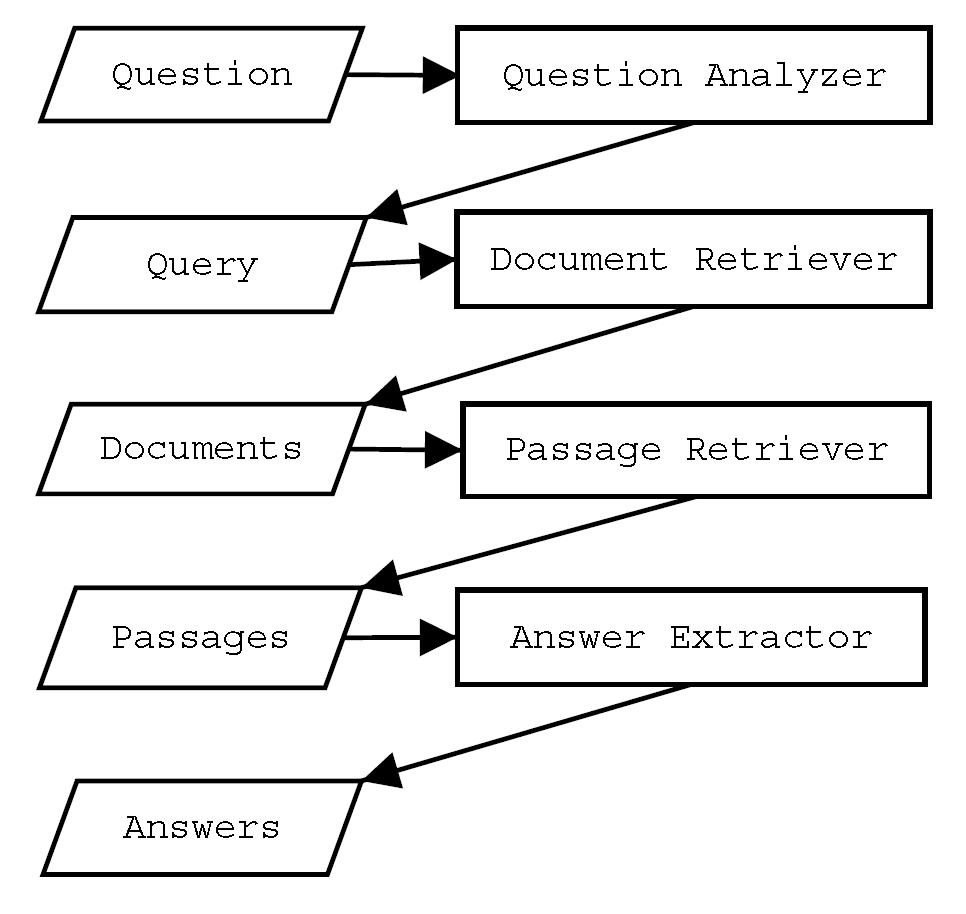
\includegraphics[scale = 0.5]{QASystem.jpg}
\caption{A typical Question Answering Architecture}
\label{fig: Question Answering Architecture}
\end{figure}

In a general question answering system, there are four major components \cite{tellex2003pmf, hirschman2002nlq,tellex2003qep, bilotti2004wbq}:

\begin{itemize}
\item {Question analysis: There are two tasks in this component. First, questions in natural language asked by a user need to be converted into queries that are needed by the subsequent parts of the system. The queries created from user's question contain terms likely to appear in documents containning an answer, for instance for such question as \textit{What is the capital of Vietnam?}, the corresponding query is \textit{capital + vietnam}. Second, the expected answer type for this question is detected in this stage so that it helps to narrow the space of searched answers. For example, questions with \textit{When} always relate to \textit{time}, thus those terms concerning time are expected such as \textit{date}, \textit{hour}, etc. }.
\item {Document retrieval: This task is to retrieve documents from the corpus that may be taken from Internet by a search engine or archived documents likely to contain answers to the query.}
\item {Passage retrieval: A passage can be simply defined as a sequence of words regardless of individual sentences or paragraphs. Some text-based information retrieval systems define a passage as a fixed-length block of words. \cite{goharian2008dsp}. Passage retrieval algorithms take a document and a question and try to return a list of passages from the document that are most likely to contain the answer information. For this,  all passages are compared with each other using passage scoring. In text-based question answering system, the score of a passage is based on the score of its words with respect to question words. The score of a question word found in a passage is calculated based on the definition of this word and/or relations of this word with other words in the text \cite{tellex2003qep}.}
\item {Answer extraction: Based on the question analysis and retrieved passages, the system extracts phrase/phrases representing an answer.}
\end{itemize}

We are only interested in the passage retrieval stage and not in the document retrieval, the question analysis nor in the answer extraction. It is because we have already had documents as meeting transcripts and the type of questions as the BET questions that are statements to be assessed. In our case, the type of answers is simply \textit{true} or \textit{false} one bit for each question. We do not need an answer as a short text extracted from the retrieved passage in which we will still have to compare two answers in order to determine the true statement. Moreover, the answer extraction is a difficult task and it can not avoid some errors. We would rather use the fully retrieved passages in determining the true statement. Thus, the stage of answer extraction is not suitable to develop in our system. For this reason, we will present only state-of-the-art methods related to passage retrieval including both traditional methods and modern methods.


Most passage retrieval algorithms calculate passage scoring based on words from the passage that are found in the question, namely matched words. However, the method of computing matched word score is different from each algorithm. 

The simplest algorithm for this approach was proposed by Light\cite{light2002aec}, in which a passage score function counts the number of words from the question found in the passage as the score for this passage. That means all words are treated equally and are given the same importance. Many question answering systems use this method as a baseline score to evaluate their performance. 

To date, there are many passage retrieval methods that have been presented in the Text Retrieval Conference (TREC) \url{http://trec.nist.gov}. These methods can be classified into two groups. One group includes traditional methods and assigns scores to each matched words independently. That means there are no relations between two matched words. Another group  considers relations amongst matched words to assign scores to them. 

For the first group, typical approaches use part-of-speech and/or frequencies of a word in order to calculate a score. Meanwhile for the second group, dependency relation among matched words in a phrase is computed to give a score for this phrase instead of words. This makes the second group more suitable to capture semantic properties than the first group.

Take SiteQ's passage retrieval algorithm \cite{lee2002seh} as an example. In this system a passage consists of some consecutive sentences segmented by punctuation and passage score is calculated by summing the weights of individual sentence in the passages. Each sentence is given a score by a formula that combines both the part-of-speech method and the query term density method. The weight of the matched words is assigned as follows: A proper noun (a common noun recognized by a capital letter) has a higher score than a verb, an adjective and/or an adverb. The term density is defined as the distance among matched words. If two sentences have the same number of matched words the sentence with smaller distance will receive a higher score.

The main idea of using word frequencies is that if a word appears many times in a current passage but only a few in other passages, its score in the current passage is higher \cite{robertson2004uid}. That means the importance of a word increases proportionally due to the number of times this word is found in a passage, but inversely to the number of times this word is found in the overall document. The simplest method for this idea is the \textit{term frequency inverse document frequency} \textit{\ensuremath{tf\times idf}}. In which, the \textit{tf} is the term frequency that measures the importance of the term \textit{\ensuremath{t_{i}}} within the document \textit{\ensuremath{d_{i}}} and \textit{idf} is the inverse document frequency that measures the importance of the term \textit{\ensuremath{t_{i}}} in the whole collection of documents. The Okapi BM25 \cite{robertson1996ot, beaulieu1995ot, xue2008rmq, comas2008sdr, tellex2003qep} presents state-of-the-art method for assigning weights to matched words using word frequencies. In fact, Okapi BM25 is a ranking function that is used to rank matching documents according to their relevance to a given query. Thus, it is often used in the Document Retrieval stage of question answering systems. However, according to the Okapi BM25 presented in the TREC-4 \cite{robertson1996ot}, this function is also used for passage determination and search. In addition, it is a complex function which was developed from the function of term frequency-inverse document frequency \textit{\ensuremath{tf\times idf}} \cite{robertson2004uid}. 

More approaches in the second group consider dependency relation among matched words, in which n-gram matching is the simplest case. The n-gram method pays more attention to the order of matching words. Accordingly, those in order are better. More specifically, this method is used to estimate similarity between two strings by examining all n-word substring matchings instead of word matchings \cite{robertson1998ang}. Another simple method is to use word density presented in the SiteQ's algorithm above. A more complex method for these approaches presented by Cui \cite{cui2005qap} uses a dependency tree to assign scores to sentences. Given the reason that one sentence in English can be written in different ways by exchanging position of words in the sentence without changing its meaning. For instance, with the sentence \textit{John wrote a science fiction book}, it may be written in some different ways but the meaning will remain unchanged. The different ways of writing the sentence include: 1)  \textit{A science fiction book was written by John}; 2) \textit{John wrote a book of science fiction}; 3) \textit{A book of science fiction was written by John}; and 4) \textit{John wrote a science fiction book}. These sentences can build a dependency tree that represents correctly positioned word relations in the sentences, so that a given query will be compared with this tree instead of one initial sentence.
 
In order to enhance the performance of question answering systems, lexical extensions for queries are added such as stemming, lemma, synonyms \cite{light2002aec}, \cite{tellex2003pmf},\cite{bilotti2004wbq}, \cite{lee2002seh}.


\chapter{Data description}

Our system is designed for data with a specific format and type so that the proposed algorithm can make use of them. In this chapter, two meeting transcripts and questions for these two meetings will be described. An analysis of this data, which gives the reasons for building our algorithm, is also presented. 

The questions used to test the system were created by the BET method. Thus, in order to have an overall view of this project as well as to understand some features of the questions, we present a brief description of the BET method and the BET question in the first part of the chapter.

\section{The BET method}
A method for meeting browser evaluation was originally proposed  by Flynn, M. and Wellner, P. \cite{flynn2003sgb} is the BET. This method evaluates a meeting browser based on user performance rather than subjective judgment. According to the BET, the act of browsing a meeting recording is an attempt to find a maximum number of \textit{observations of interest} in a minimum amount of time \cite{BET}, in which \textit{observations of interest} are defined as interesting to the meeting participants or to people who missed the meeting. Thus, the task of evaluating of a meeting browser is to collect a set of \textit{observations of interest} and then ask human subjects to verify these observations as binary-choice test questions in a fixed amount of time by using a meeting browser to access the meeting. A \textit{good} meeting browser will help human subjects find as many correct answers as possible in a shortest amount of time. Information on human subjects is collected as answer precision (known as \textit{effectiveness}) and answer speed (known as \textit{efficiency}) and is used to evaluate the performance of the meeting browser. In detail, an \textit{observation of interest} is formed as a complementary pair of statements, one true and one false about a fact related to a meeting recording and human subjects are asked to determine which statement is true and which statement is false in the pair. The answer precision is calculated by dividing the number of correct answers over total answers. In terms of the answering speed, it is computed as the average time required to answer a question. Analyzing this information and comparing it among different meeting browsers provides scores for the performance of a meeting browser.

This is a time-consuming method that requires investment in collecting, preparing the observation and performing experiments with subjects. However, this observation collection is independent to browsers so that the collected observations can be extended to be used for the evaluation of other meeting browsers in the future. \cite{BET4TQB}.

The stages of the BET method are presented in the Figure \ref{fig1: BET stages}.

\begin{figure}[htbp]
\centering
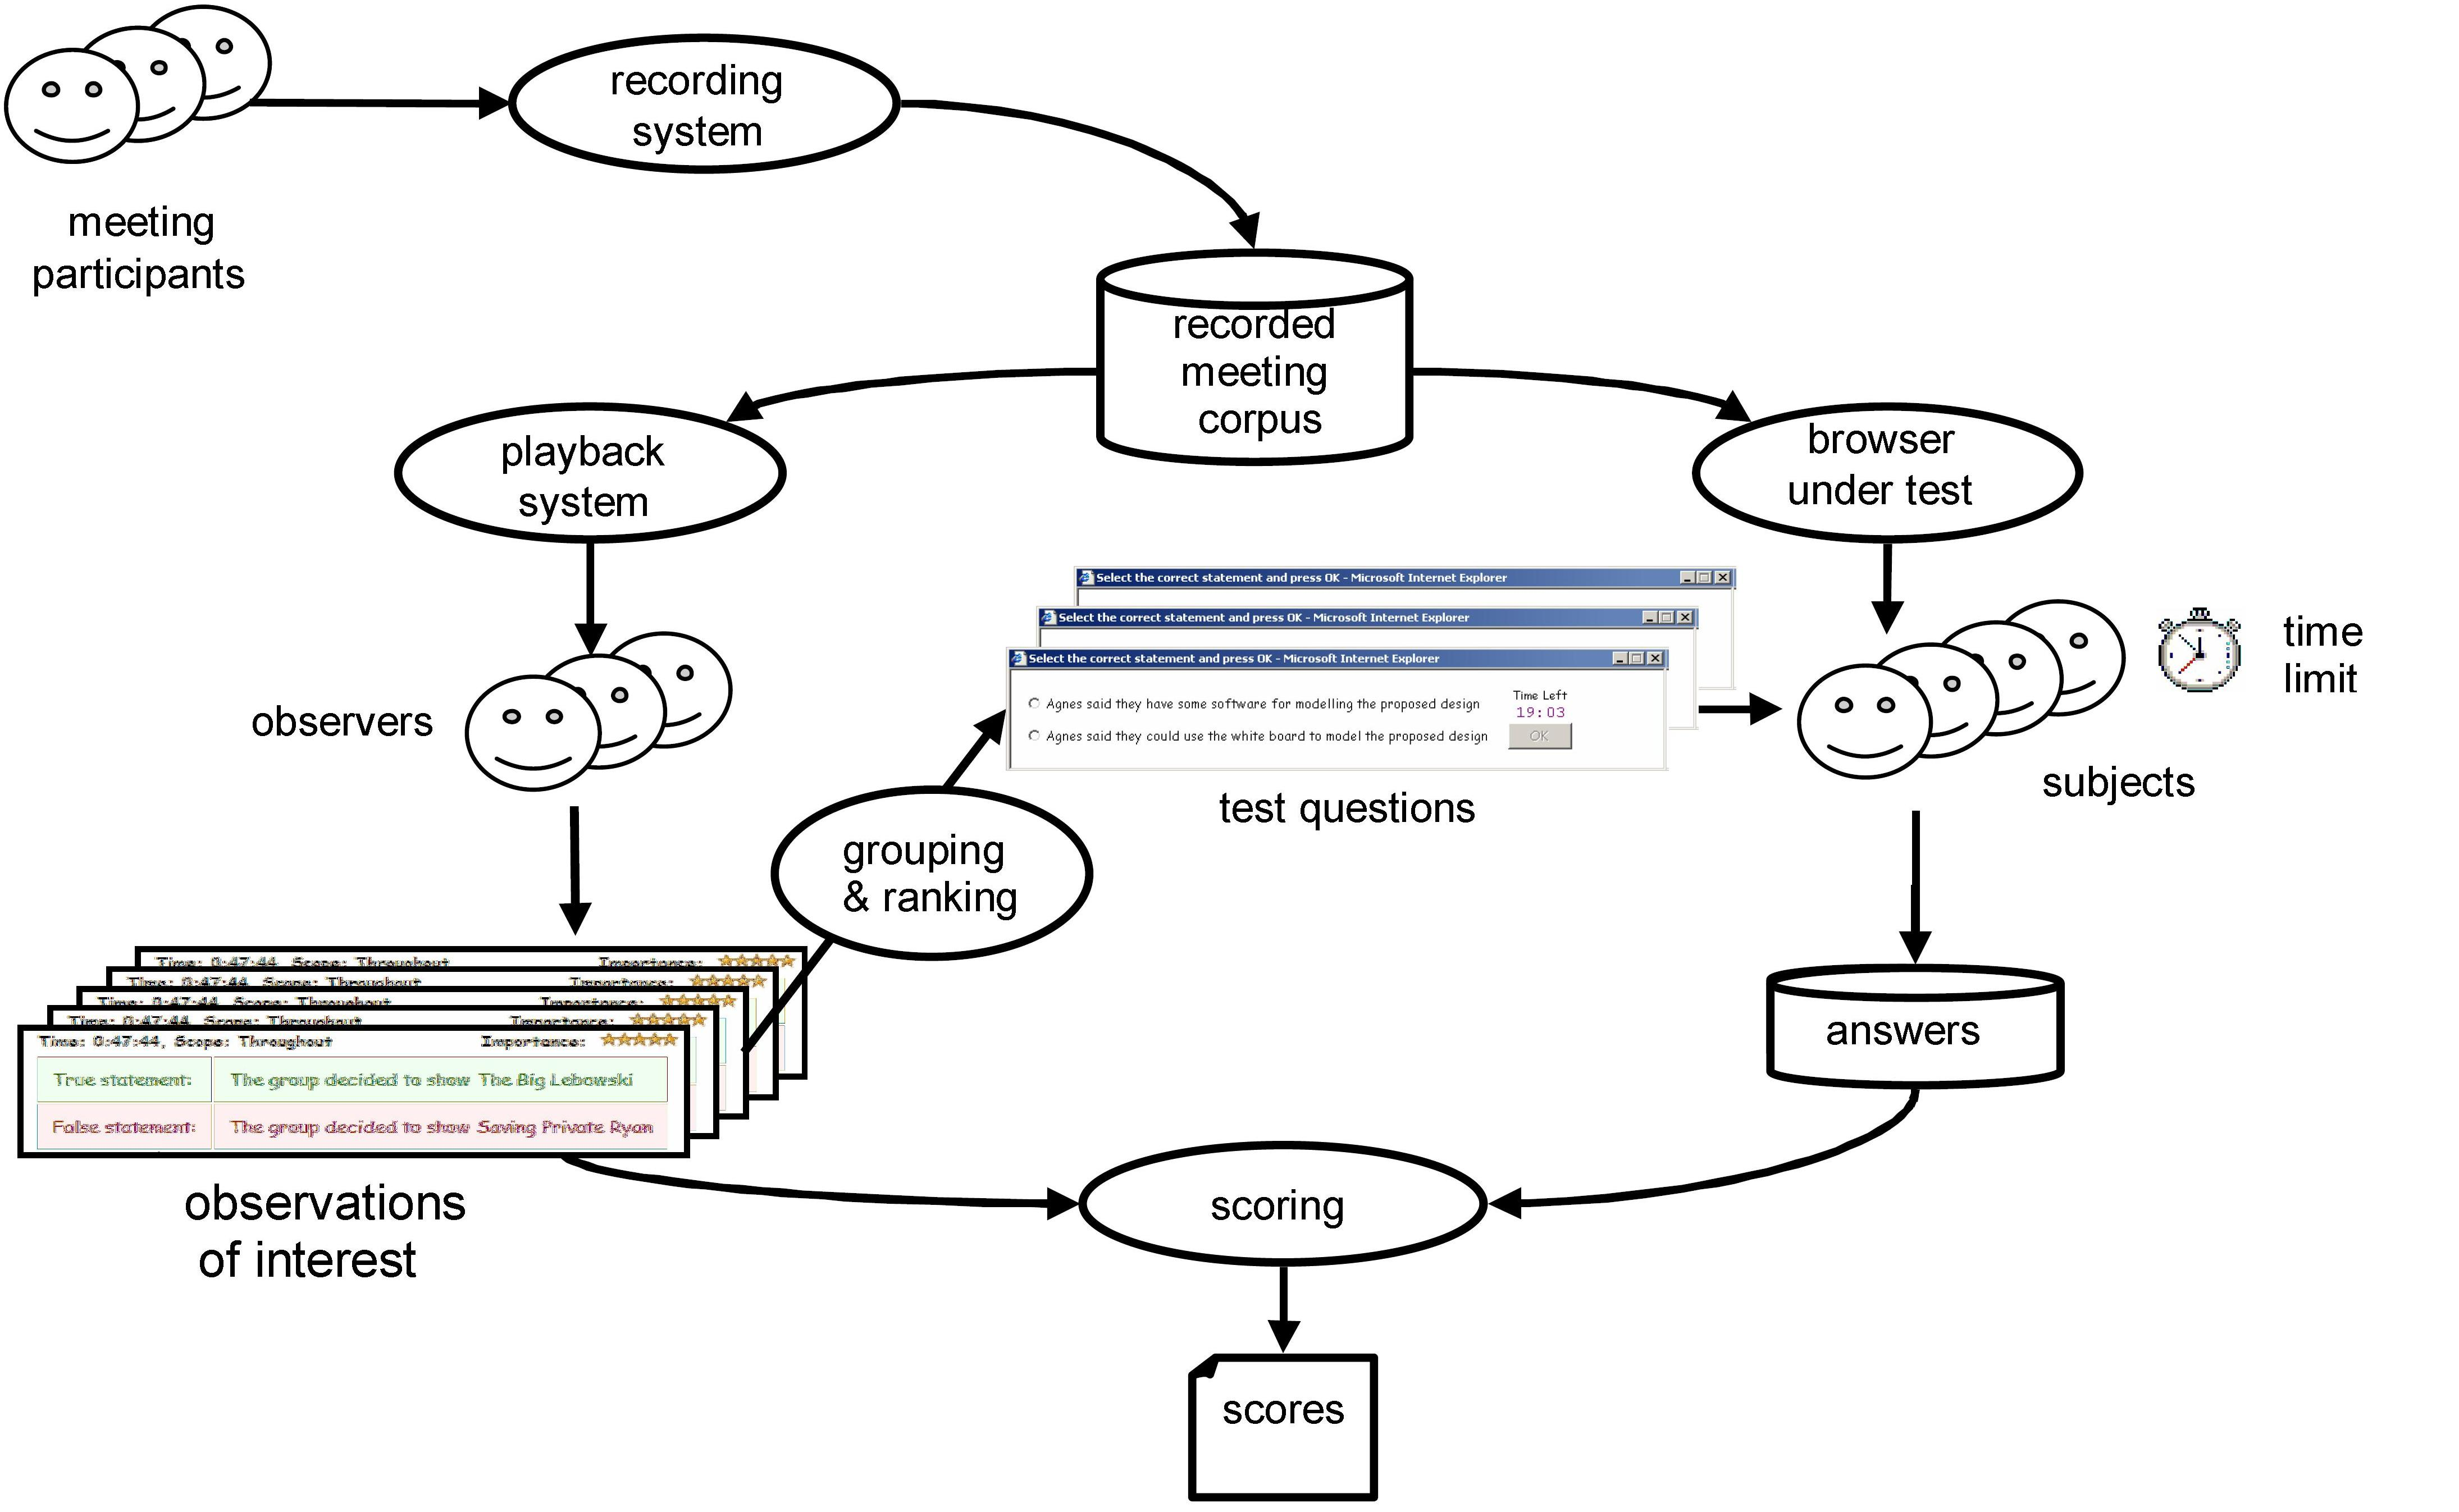
\includegraphics[scale = 0.15]{BET_stages.jpg}
\caption{Stages in the design and execution of a BET evaluation \cite{popescubelis:tbe}}\label{fig1: BET stages}
\end{figure}

\section{The BET Questions}
The pairs of statements used for the BET method, called the BET questions, are produced by a set of neutral observers, who independently watch selected meetings from corpus. These observers are native English speakers from the University of Sheffield. They are students, researchers and lecturers. The observers have unlimited time and access to the full recordings from such media sources as videos, audios, in parallel with paper printouts of the slides that participants worked on for the meeting. At first, an observer collects a list of observations that are true statements about facts or events that may interest meeting participants or people who missed the meeting. The collected statements should not be easy to guess without using the meeting information.  Then, for each true statement, a false counterpart statement is created so that a pair of complementary statements are generated. The observations should be simple and concisely stated.


An interface for observation collection is presented in the Figure \ref{fig2: create observations}. As seen in the Figure, there are three buttons \textit{Nearby}, \textit{Around} and \textit{Throughout} that indicate the position of information required to answer the question in the transcript. One observation is marked as \textit{Nearby} or \textit{Here} if it is pertinent to that particular moment; marked as \textit{Around} if it covers at least a minute of the meeting around the point the observers have selected; and marked as \textit{Throughout} if it broadly covers the whole meeting. However, in this system, the questions whose type is \textit{Throughout} are avoided because it is difficult to determine relevant passages which contain information required to  answer the questions using an automatic system. After that, the collected observations are examined by experts to reject repeated or inappropriate ones. 

\begin{figure}[htbp]
\centering
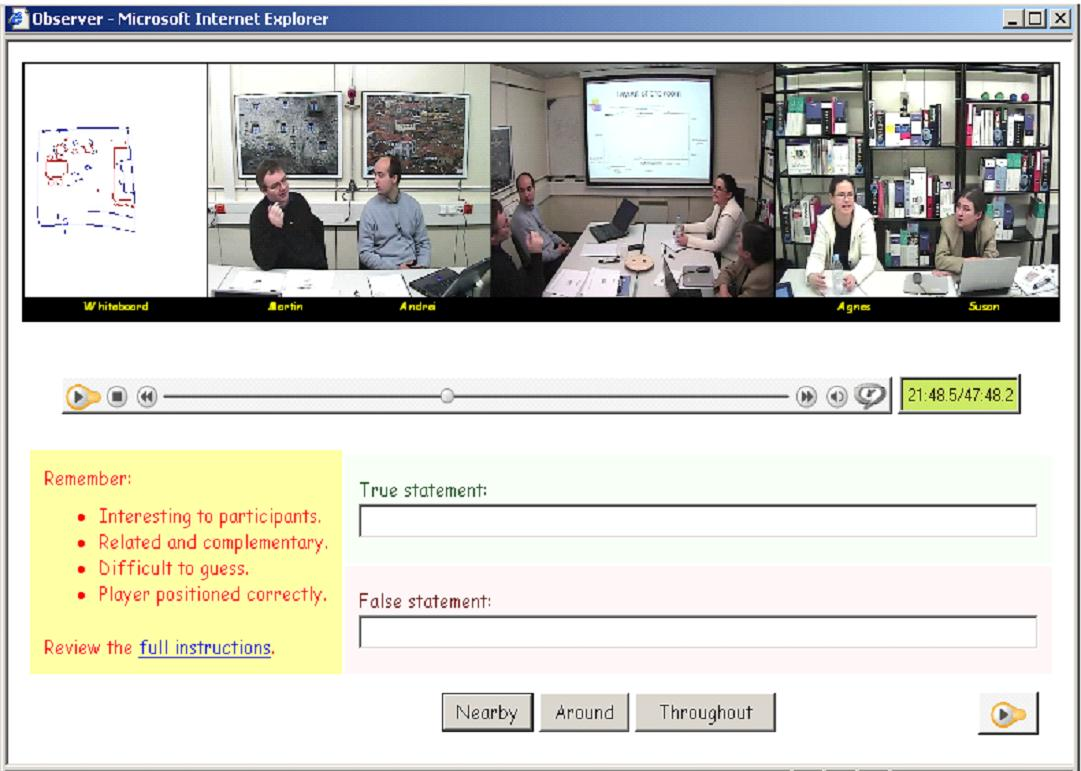
\includegraphics[scale = 0.5]{BET_interface.jpg}
\caption{Interface for observers}\label{fig2: create observations}
\end{figure}


\section{Data used to test the system}
\subsection*{Meeting transcripts}

Two meeting transcripts used to test the system were taken from the corpus built by the AMI project \cite{AMI_corpus}. Both of them are in English, involving four participants, native or non-native English speakers. The first meeting, IB4010, lasted 50 minutes in which managers of a movie club discussed how to select the movie for the next show. In the second meeting, IS1008c, a team discussed the design of a remote control for 26 minutes. There are two versions of the meeting transcripts, including manual and automatic ones. 

Unnecessary information from the original transcripts from AMI Corpus was eliminated such as time of utterances and notations of episodes. Consequently, the most important information left in the two manual meeting transcripts is speaker name and utterances that are showed in the Tables \ref{transcript_IB4010} and \ref{transcript_IS1008c}.

In a conversational document such as a meeting transcript, information about speakers plays an important role in answering the questions that verify a statement with respect to the speaker of one/some utterances. That is why in the proposed algorithm, in order to calculate passage scoring, we pay more attention to the name of speakers in both questions and transcript. For instance, score for a matched word as speaker name is the highest compared to other matched words.


%\begin{table}[htbp]
%\footnotesize
%\caption{Description of meeting transcript}
%\begin{center}
%\begin{tabular}{|lp{5cm}|lp{5cm}|}
%\hline
%\multicolumn{ 2}{|c|}{\textbf{Movie club meeting (IB4010)}} & \multicolumn{ 2}{c|}{\textbf{Remote control design meeting (IS1008c)}} \\ \hline
%\multicolumn{1}{|c}{\textbf{Speaker}} & \multicolumn{1}{c|}{\textbf{Utterances}} & \multicolumn{1}{c}{\textbf{Speaker}} & \multicolumn{1}{c|}{\textbf{Utterances}} \\ \hline
%Andrei  & Hi everyone.  & Sridhar  & so if you find out from the technology background, okay, so that would be good.  \\ 
%Denis  & So I don't know if you all received the the a- agenda for this meeting.  Do you - no?  & Christine  & Sounds good.  \\ 
%Mirek  & No, I haven't.  & Agnes  & Why was the plastic eliminated as a possible material?  \\ 
%Denis  & Here it is.  & Christine  & Because um it gets brittle, .. cracks -  \\ 
%Mirek  & Thank you.  & Christine  & We want - we expect these um uh these remote controls to be around for several hundred years.  Good expression.  \\ 
%Agnes  & I haven't.  & Ed  & Good expression.  \\ 
%Denis  & So um um the goal for today are um - We have two goals. Uh - First is to decide a movie for uh the next projection for our movie club.  & Christine  & I don't know, speak for yourself, I'm planning to be around for a while.  \\ 
%Mirek  & Mm-hmm.  & Agnes  & Although I think - \$ I think with wood though you'd run into the same types of problems, wouldn't you? I mean, it chips, it- if you drop it, uh it's - I'm not sure \$  \\ 
%Andrei  & Mm-hmm.  & Sridhar  & So so you're not convinced* about the the wood, yes.  \\ 
%... & ... & ... & ... \\ \hline
%\end{tabular}
%\end{center}
%\label{Meeting transcript}
%\end{table}


\begin{table}[htbp]
\caption{Meeting transcript IB4010}
\begin{tabular}{|lp{12cm}|lp{0cm}|}
\hline
Andrei & Hi everyone. \\
Denis & So I don't know if you all received the the a- agenda for this meet-
ing. Do you � no? \\ 
Mirek & No, I haven't. \\ 
Denis & Here it is. \\
Mirek & Thank you. \\
Agnes & I haven't. \\ 
Denis & So um um the goal for today are um - We have two goals. Uh - First is to decide a movie for uh the next projection for our movie club. \\ 
Mirek & Mm-hmm. \\ 
Andrei & Mm-hmm. \\   \hline
\end{tabular}
\label{transcript_IB4010}
\end{table}


\begin{table}[htbp]
\caption{Meeting transcript IS1008c}
\begin{tabular}{|lp{12cm}|lp{0cm}|}
\hline
Agnes & Why was the plastic eliminated as a possible material? \\
Christine & Because um it gets brittle, .. Cracks �  We want - we expect these um uh these remote controls to be around for several hundred years. 
Good expression. \\ 
Ed & Good expression. \\ 
Christine & I don't know, speak for yourself, I'm planning to be around for a while. \\ 
Agnes & Although I think - \$ I think with wood though you'd run into the same types of problems, wouldn't you? I mean, it chips, it- if you drop it, uh it's - I'm not Sure \$ \\ 
Sridhar & So so you're not convinced* about the the wood, yes. \\  \hline
\end{tabular}
\label{transcript_IS1008c}
\end{table}



\subsection*{Questions}

The BET questions were mentioned above. However, some information of the questions used in this system is eliminated from full versions of original BET questions, which consist of miscellaneous information such as observation time, mediate time, important level, scope, etc. \cite{BET}.  The system needs only the true and the false statement in each question, which are considered as input data to distinguish one from another. Examples of some pairs are in the Tables \ref{questions_IB4010} and \ref{questions_IS1008c}.


For the two meetings IB4010 and IS1008c, 222 and 217 raw observations were collected by 9 and 6 observers respectively. After being filtered and corrected, the results are only 116 and 50 final pairs of true/false statements.

\begin{table}[htbp]
\caption{The BET questions IB4010}
\begin{tabular}{|lp{12cm}|lp{0cm}|}
\hline
True & Mirek had not received the agenda for the meeting \\
False & Andrei had not received the agenda for the meeting \\ \hline
True & None has seen the Shawshank redemption \\ 
False & Only two have seen the Shawshank redemption \\ \hline
True & Denis informed the team that the first objective was to choose a film and the second was
to discuss an advertising poster \\ 
False & Denis informed the team that the first objective was to choose a film and the second was to discuss a date for the film to be shown \\ \hline
\end{tabular}
\label{questions_IB4010}
\end{table}

\begin{table}[htbp]
\caption{The BET questions IS1008c}
\begin{tabular}{|lp{12cm}|lp{0cm}|}
\hline
True & One of the features under consideration is speech recognition. \\ 
False & One of the features under consideration is fingerprint identification. \\ \hline
True & The product is expected to last over several hundred years. \\ 
False & The product is expected to last more than 5 but less than 15 years. \\ \hline
True & Christine eliminated plastic as too brittle over time. \\ 
False & Christine eliminated plastic as it would flex and damage the chips.  \\ \hline
\end{tabular}
\label{questions_IS1008c}
\end{table}


%\begin{table}[htbp]
%\footnotesize
%\caption{Description of the BET Questions}
%\begin{center}
%\begin{tabular}{|l|p{7cm}|p{7cm}|}
%\hline
% & \textbf{Movie club meeting (IB4010)} & \textbf{Remote control design meeting (IS1008c)} \\ \hline
%True & Mirek had not received the agenda for the meeting & One of the features under consideration is speech recognition. \\ 
%False & Andrei had not received the agenda for the meeting & One of the features under consideration is fingerprint identification. \\ \hline
%True & None has seen the Shawshank redemption & The product is expected to last over several hundred years. \\ 
%False & Only two have seen the Shawshank redemption & The product is expected to last more than 5 but less than 15 years. \\ \hline
%True & Denis informed the team that the first objective was to choose a film and the second was to discuss an advertising poster & Christine eliminated plastic as too brittle over time. \\ 
%False & Denis informed the team that the first objective was to choose a film and the second was to discuss a date for the film to be shown & Christine eliminated plastic as it would flex and damage the chips \\ \hline
%... & ... & ... \\ \hline
%\end{tabular}
%\end{center}
%\label{The BET Questions}
%\end{table}

The fact that the questions considered as statements is one main feature that makes this system different from other question answering systems, which normally consist of different questions like \textit{How}, \textit{Why}, \textit{When}, etc. For this reason, it is not necessary to apply an existing complex algorithm, which was widely used to deal with various type of questions in other question answering systems. Therefore, our proposed algorithm is designed to try to fit the type of the BET questions. In this case, a typical question ask to verify information spoken by a speaker, for instance \textit{Mirek asks who has seen Schindlers List}. In this case, they have a speaker name at the beginning of the sentence. According to our statistics, there are over 55\% of such questions (28/50 such questions for IS1008c and 87/116 such questions for IB4010). This is an important remark that score of one matched word spoken by speaker whose name is mentioned in both the transcript and the question should be higher than other matched words.

Another feature of the questions is the similarity of two statements in a pair. In most pairs, two statements are different from each other by only one or two words. Therefore, at the Passage Retrieval stage of the proposed algorithm, the probability that the two found corresponding passages coincide is very high. In this case, the true and the false statement can be distinguished by the similarity between each candidate statement with the corresponding passage. In other words, passage score for each statement is compared to determine the true statement/the false statement.

%Remain questions seem to be straightforward.

\chapter{Proposed algorithm}


The proposed algorithm was developed using lexical similarity algorithm combined with some of existing techniques, which are n-gram matching, lexical extensions. However, the way of computing passage scoring pays more attention to the specifications of meeting transcripts, which will be presented in detailed in the following sections.

Our system proceeds in three stages: (i) In the first stage, known as a pre-processing, the two questions and meeting transcripts are normalized and reorganized in order to enhance the performance of the algorithm; (ii) The second stage identifies a section of the meeting transcript which is most likely to contain the answer (i.e. evidence deciding the true and the false statement); and (iii) The third stage compares the two candidate statements with respect to the identified paragraph(s), and returns the true one. 


Figure \ref{SystemOverview} gives an overview of the 3 stages.

\begin{figure}[htbp]
\centering
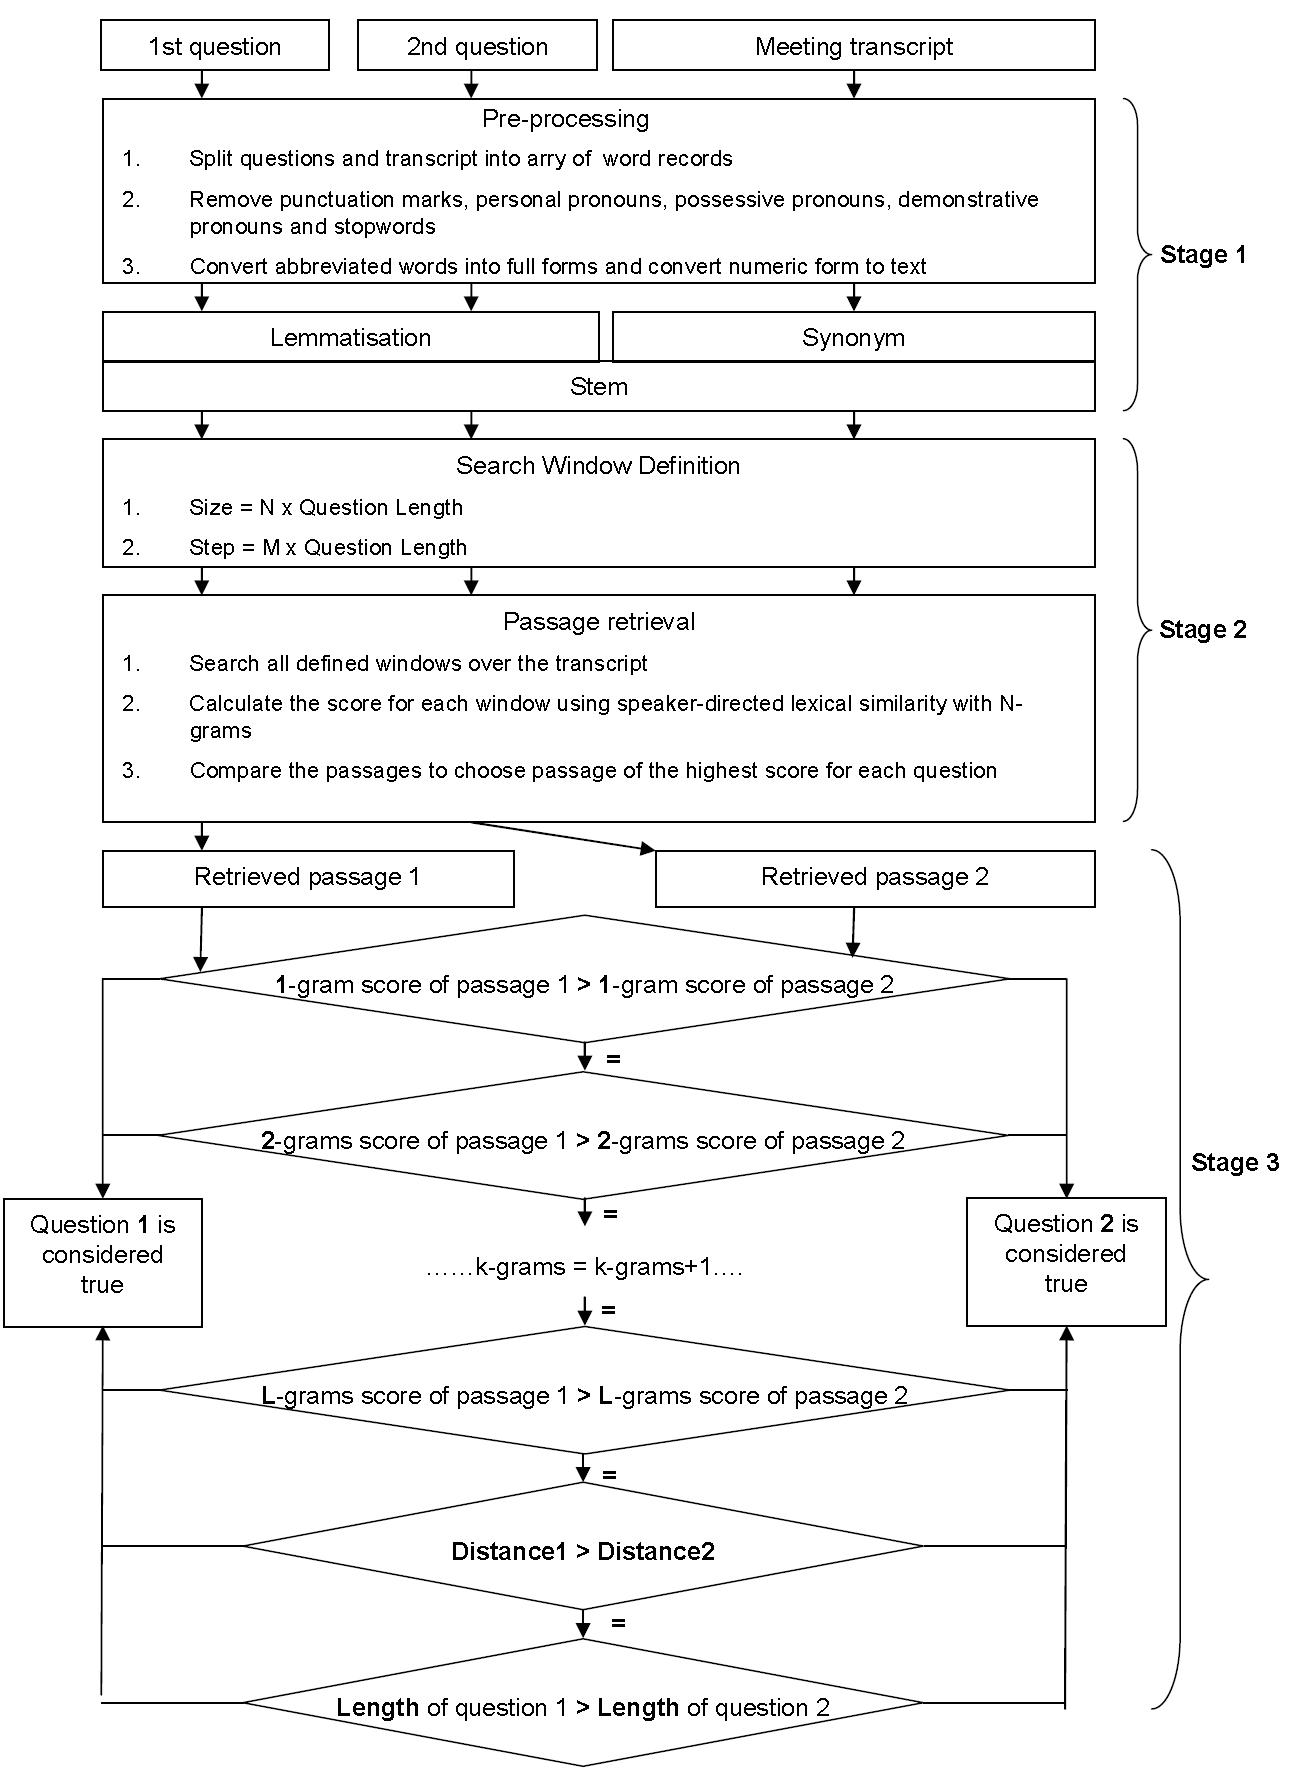
\includegraphics[scale = 0.6]{Stages_of_system.jpg}
\caption{Overview of the system}\label{SystemOverview}
\end{figure}


%Figure \ref{SystemOverview}



\section{Pre-processing}
There are two main tasks for this section. First, questions and transcript are transformed into the same form of written text so that they can be compared word by word later. Secondly, in order to enhance the probability of matching between two words, each word is extended by lemma, stem and synonyms.

The first processing is done by five operations as follows:

\begin{enumerate}
\item {Removing characters as punctuation marks: comma, dot, quotation mark, semicolon or exclamation, \ldots because these characters do not have any effects on the proposed algorithm based on lexical similarity. } 

\item {Removing stopwords such as "the", "to" or "for" that generally add little or no information regarding the subject matter of text \cite{mckechnie2001cap}.  This helps to reduce cost of computing as well as to take precaution that they muddle the signal from the more content words \cite{hirschman1999drr}}

\item {For the reason that the questions are indirect-speech statements meanwhile the the meeting transcript is a direct-speech report, words that may be changed for a transformation from direct speech to indirect speech should be avoided from counting matched words between a question and a passage because this leads to lexical mismatches. They are personal pronouns (I, me, myself, you, \ldots), possessive pronouns (my, your, \ldots), demonstrative pronouns (this, that, \ldots).}



\item {Converting numeric forms to text forms: 34 \ensuremath{\rightarrow} thirty four, 2nd \ensuremath{\rightarrow} second, etc. \ldots so that they are written in the same way, this prevents an unnoticed matching while the algorithm executes. }

\item {Converting abbreviated words into full forms: We've \ensuremath{\rightarrow} We have, I'll \ensuremath{\rightarrow} I will, etc. \ldots. This operation helps the system treat the text in the same way.}
\end{enumerate}

All words are transformed into lower-case forms so that nouns, pronouns and verbs have the same level of importance. That means parts-of-speech will not be used to assign scores to words in the Passage Retrieval stage.

The proposed algorithm uses lexical similarity to find a relevant passage that contains answer information (Section 4.2). Thus, a lexical extension should be added so that the system has more than one matching possibility between two words. Take the words \textit{production} and \textit{product} as examples, they match each other because they have the same stem as \textit{produc}.

Three lexical extensions are added to each word, including lemma, stem and synonym. 
\begin{itemize}
%\item {Lemma is the canonical form of the word.}
\item {A stem or word stem is a root or roots of a word that is common to all its inflected variants \cite{Stem}.}
\item {A lemma in morphology is defined as a canonical form of a set of words that have the same original meaning \cite{clement2004mba}. A lemma is different from a stem in which a lemma of the verb may change when morphologically inflected, however a stem that never changes by doing a morphology. For example, for the word "modified", its lemma is "modify" while the stem is "modifi" because we have words such as \textbf{modifi}cation (done by WordNet\cite{miller1995wld}).}
\item {A synonym of a word is another word that they share at least one sense in common \cite{miller1995wld}.}
\end{itemize}

However, it is not suitable to apply all these extensions to both questions and the transcript. For instance, if both question words and answer word are extended by a set of synonyms, it can create a so called "redundant information". In addition, it may make the result of the algorithm inaccurate if they are considered similar because of similarity of an intermediate synonym. For example: \textit{meeting} and \textit{challenge} have one synonym \textit{contest} in common, but they do not have the same meaning. For that reason, a question word is extended by adding its lemma, meanwhile the transcript words are extended by adding a set of synonyms. Meanwhile, stem is applied as the last operation on each word. This may increase the signal from words. For instance with such a question word as the verb \textit{modified} and such a transcript word as the noun \textit{modification}, there are not any matching between these words, even after adding a lemma and a synonym.  In detail, \textit{modified} becomes \textit{modify} by a lemmatisation and \textit{modification} has five synonyms \textit{alteration, adjustment, qualifying, limiting, change} (returned by WordNet \cite{pasca2001irw}). But after stemming by Snowball \cite{porter2001ss}, these two words will have a same form as \textit{modifi}, so they are matched.

In practice, for each word, the program runs a Stemming API of Porter, called Snowball \cite{porter2001ss} to obtain a stem and WordNet API \cite{pasca2001irw} to obtain a lemma and a set of synonyms.

A set of synonyms is reduced to be more coherent with the original word by using parts of speech (PoS) tool named QTAG tagger \cite{manson1997qpp}, which aims at removing synonyms that do not have the same PoS as the original word. A PoS tagger is an algorithm that reads text and for each token in the text returns the text-tokens part-of-speech, e.g. noun, verb or punctuation. 

Therefore, each word will be treated from now on as a record of many fields. For a question word, it has three fields: original word, lemma of the word and stem of the lemma. They are described in the Table \ref{Word splitting and lexical extensions for questions}. The format of input transcript as described in the Tables \ref{transcript_IB4010} and \ref{transcript_IS1008c} helps the program identify the speaker of any word in the transcript. Hence, a record of a transcript word has five fields: original word, stem of word, name of speaker name who spoke this word, set of synonyms and part of speech. They are described in the Table \ref{word_splitting_transcript}. The name of speakers is also stemmed in order to compare with a question word which may be a speaker name. This field is very important to assess a statement with respect to a specific speaker.

The fields \textit{synonyms} and \textit{lemma} are structured as a set of words because they may have more than one element. For example, lemma of "better" has two words \textit{good} and \textit{well}, synonyms of \textit{better} are \textit{break}, \textit{improve}, \textit{amend}, \textit{ameliorate} and \textit{meliorate}.


For instance, for the pair of such questions as \textit{Mirek had not received the agenda for the meeting} and \textit{Andrei had not received the agenda for the meeting}, after removing stop-words, they remain \textit{Mirek had not received agenda meeting} and \textit{Andrei had not received agenda meeting}. Their lexical extensions are presented as following tables:
%\begin{table}[htbp]
%\scriptsize
%\caption{Word splitting and lexical extensions for questions}
%\begin{tabular}{|c|l|l|l|l|c|l|l|l|}
%\hline
%\multicolumn{ 4}{|c|}{\textbf{Question 1}} &  & \multicolumn{ 4}{c|}{\textbf{Question 2}} \\ \hline
%\textbf{Position} & \multicolumn{1}{c|}{\textbf{Word}} & \multicolumn{1}{c|}{\textbf{Lemma}} & \multicolumn{1}{c|}{\textbf{Stem}} &  & \textbf{Position} & \multicolumn{1}{c|}{\textbf{Word}} & \multicolumn{1}{c|}{\textbf{Lemma}} & \multicolumn{1}{c|}{\textbf{Stem}} \\ \hline
%1 & Mirek & Mirek & Mirek &  & 1 & Andrei & Andrei & Andrei \\ \hline
%2 & had & have & have &  & 2 & had & have & have \\ \hline
%3 & not & not & not &  & 3 & not & not & not \\ \hline
%4 & received & receive & receiv &  & 4 & received & receive & receiv \\ \hline
%5 & agenda & agenda & agenda &  & 5 & agenda & agenda & agenda \\ \hline
%6 & meeting & meet & meet &  & 6 & meeting & meet & meet \\ \hline
%\end{tabular}
%\label{Word splitting and lexical extensions for questions}
%\end{table}


\begin{table}[htbp]
\scriptsize
\begin{center}
\caption{Word splitting and lexical extensions for the first question}
\begin{tabular}{|c|l|l|l|}
\hline
\textbf{Position} & \multicolumn{1}{c|}{\textbf{Word}} & \multicolumn{1}{c|}{\textbf{Lemma}} & \multicolumn{1}{c|}{\textbf{Stem}} \\ \hline
1 & Mirek & Mirek & Mirek \\ \hline
2 & had & have & have \\ \hline
3 & not & not & not \\ \hline
4 & received & receive & receiv \\ \hline
5 & agenda & agenda & agenda \\ \hline
5 & meeting & meet & meet \\ \hline
\end{tabular}
\label{question1}
\end{center}
\end{table}



\begin{table}[htbp]
\begin{center}
\scriptsize
\caption{Word splitting and lexical extensions for the second question}
\begin{tabular}{|c|l|l|l|}
\hline
\textbf{Position} & \multicolumn{1}{c|}{\textbf{Word}} & \multicolumn{1}{c|}{\textbf{Lemma}} & \multicolumn{1}{c|}{\textbf{Stem}} \\ \hline
1 & Andrei & Andrei & Andrei \\ \hline
2 & had & have & have \\ \hline
3 & not & not & not \\ \hline
4 & received & receive & receiv \\ \hline
5 & agenda & agenda & agenda \\ \hline
5 & meeting & meet & meet \\ \hline
\end{tabular}
\label{question2}
\end{center}
\end{table}

\normalsize



One example for a snippet of transcript as below:
\scriptsize
\begin{verbatim}
.....
 Andrei Hi everyone. 
 Denis  So I don't know if you all received the the a- agenda for this meeting.
 Denis 	Do you - no?
 Mirek 	No, I haven't.
....
\end{verbatim}
\normalsize

After the processing, it remains:
\scriptsize
\begin{verbatim}
.....
denis   9 not 10 know 11 if 12 you 13 all 14 received 18 agenda 21 meeting
denis   24 no 
mirek   25 No 27 have 28 not
....
\end{verbatim}
\normalsize

and it is transformed into the following table:

\begin{center}
\begin{threeparttable}
\scriptsize
\caption{Word splitting and lexical extensions for transcript (see Appendix \ref{PoS} for the explanation of PoS tags)}
\label{word_splitting_transcript}
\begin{tabular}{|c|l|l|c|l|l|}
%\hline \multicolumn{6}{|c|}{Word splitting} \\
\hline  \bf{Position} & \bf{Word} & \bf{Stem} & \bf{Speaker} & \bf{Synonyms (stemmed)} &\bf{PoS} \\
\hline \ldots & \ldots & & & &\\
\hline 9 & not & not & deni & non & NOT\\
\hline 10 & know & know & deni & cogniz experi live acknowledg recogn \ldots & VB\\
\hline 11 & if & if & deni & & CS\\
\hline 13 & all & all & deni & entir complet total altogeth whole  \ldots & PDT\\
\hline 14 & received & receiv & deni & have get find obtain \ldots &VBD\\
\hline 18 & agenda & agenda & deni & docket schedul agendum \ldots & NN\\
\hline 21 & meeting & meet & deni & fill match ensembl contact \ldots & NN\\
\hline 24 & no & no & deni & nobelium & DT\\
\hline 25 & no & no & mirek & nobelium & DT\\
\hline 27 & have &have &mirek &  receiv get own possess \ldots &HV\\
\hline 28 & not &not &mirek & non&XNOT\\
\hline \ldots & \ldots & & & &\\
\hline 
\end{tabular}
\end{threeparttable}
\end{center}


\normalsize

All of the steps above are processed in a procedure separated from execution of the main algorithm, which consists of passage retrieval and true-false answer. The questions and the transcript pre-processed from this stage are stored on hard disk so that the programme can load them into RAM before running the main algorithm. This saves us much time to experiment on different configurations of the algorithm that requires the repeatition of execution with the same input data. 

\section{Passage retrieval} 

% definition of a passage must be mentioned in the state-of-the-art

The main goal of this stage is to narrow the space of searched answer by locating a passage which is considered the most likely to contain all the information about the answer, like evidence that helps to discriminate the true statement from the false statement in a pair. It also gives a numeric score indicating the similarity level between a found passage and the question so that two complementary statements in a pair may be compared in the subsequent stage.

In order to find the relevant passage, the system has to compare all possible passages in the transcript. Information being compared is passage scoring, which is a numeric value used to measure the level of similarity between a passage and a question. This task is done by moving a search window from one place to another over the entire transcript. If we assume that the transcript is a cloth stretched to be ironed, then the search window is the iron. In the same way of using an iron, the search window passes over all possible passages that have the same size as the search window in the transcript. All of the retrieved passages by this way are compared in order to provide the passages of highest score \cite{lequocanh, lequocanh1}. 

As listed in the Chapter 2, there are many ways to calculate the score of a passage with respect to the question. According to the experimental results of Stefanie \cite{tellex2003qep} with different algorithms of passage retrieval, the performance of the algorithms is different from each other depending on input data. That means each method is suitable for only certain cases. Moreover, existing passage retrieval algorithms use input retrieved by a document retrieval that returns unknown-typed documents such as a forum website, a commercial website or an online newspaper, etc. Additionally, these approaches have to analyze the type of questions such as \textit{How} or \textit{When} before the stage of passage retrieval  \cite{TREC8, TREC2001, hirschman2002nlq, tellex2003qep}. This effects the final results of the passage retrieval algorithm because each step accumulates a certain error. In our case, the type of document and the type of questions are defined before, as described in Chapter 3. That is why we do not apply any existing complex algorithms, but rather develop our own algorithm based on the basic one presented by Light et al. \cite{light2002aec}. The method of Light is the simplest method to calculate a passage scoring, which is the number of matched words between the passage and the question. Based on this method, we added some certain extensions to the original algorithm, including n-gram matching, lemmatisation, stem, synonyms and various scores assigned to matched word. Lexical extensions such as lemmatisation, stem and synonyms have been presented in the previous stage while the application of n-gram matching and different scores are to be explained specifically in following sections \cite{lequocanh1}.

As described by Light et al, the score of a passage is based on the number of matched words. However, there are three score levels assigned to matched words. As illustrated in the table \ref{word_splitting_transcript}, each word from the transcript corresponds to one speaker's name. Therefore, if a matched word is spoken by a speaker whose name is addressed in the question, the score assigned to this word must be higher than other matched words. 

In our experiment system, as presented in the pseudo code \ref{alg: Passage Score}, different values of score are assigned to a matched word as follows: 
\begin{enumerate}
\item {If a word from the question matches the name of the speaker in the passage, then it receives the highest score (e.g., 4.0)}
\item {If a word from the question matches a word from the passage (lemmas), and this word is spoken by a speaker mentioned in the question, then it receives the second highest score (e.g.,2.5)}
\item{Otherwise, if a word from the question matches a word from the passage (lemmas) then it receives the "normal score" (e.g.,1.0)}
\item{If a word (lemma) from the question matches one of the synonyms of a word from the passage, then it receives a "low" score (e.g.,0.5)}
\end{enumerate}

The numeric values listed above are set by the author based on the intuition about the importance of each matching, and might not be optimal for this task. No automatic optimization (statistical learning) could have been attempted because the amount of data was insufficient.


As mentioned above, a search window is used to seek and calculate all possible passages on the transcript. The size of the search window is defined as a multiple of the question length. Meanwhile, the distance between two consecutive windows is known as window step and also defined as a multiple of question length. For instance, window size = 5 x question size and window step = 2 x question size. Thus, parameters of search window are dynamic depending on the input question length. This method seems suitable to retrieve relevant passages using the lexical similarity algorithm because when the length of the question increases, the information that the question demands is larger. As a result, it is necessary to enlarge the size of search window.

The passage retrieval algorithm returns a list of passages at the same highest score. Nevertheless, we would like only one passage for the next stage of the algorithm because it is likely that only one relevant passage corresponds to each BET question. In order to choose the most relevant passage, 2-gram score, 3-gram score and so on until n-gram score are compared to reduce the number of passages in the returned list, in which n is the number of question words. 

For instance, for the question \textit{Denis have seen this nice movie}, two passages \textit{All of them have seen this movie } and \textit{This movie is nice to see} have the same number of 1-gram matching words. The 1-gram matching words for the first passage are \textit{have, seen, this, movie} and for the second passage are \textit{this, movie, nice, see}. However, they have not the same 2-gram matching words. For the first passage, the 2-gram matching words are \textit{have seen, seen this} meanwhile there is no 2-gram matching words for the second passage. Thus, in this case, we can conlude that the first passage is more relevant for the question. 

A k-gram score is calculated as follows: Instead of working with matched words between question and answer, the program will work with matched substrings of k words between them. If two passages have same 1-gram score, their 2-gram score are compared with each other to return higher-score passages. If they have the same 2-gram score, their 3-gram score are compared with each other. This continues in the same way until one passage has a higher score than others or all n-gram scores are compared with each other, in which n is the number of words in the question. If they still have same n-gram score, the first passage is returned. In fact, n-gram matching is the simpler variant of the dependency relation approach among matched words that the matching of words in order is better.



The implementation of passage scoring calculation is described by pseudo code \ref{alg: Passage Score} with comments in detail. The following is a list of the most impotant features of this implementation:

- A passage is defined as a class that has 5 properties: 1) Passage score, which indicates the similarity between this passage and the current question. The passage score is computed as the sum of the scores for each matched word; 2) Position of the passage in the transcript; 3) Size of passage; 4) Set of positions of matched words in the transcript; and 5) Distance among matched words (density). This distance is calculated as the sum of absolute distance between any two matched words. This task is done at the end of the passage retrieval to prepare for the True-False Answer stage.


- The order of priority is to "name matching", then "stem matching" and lastly "synonyms matching" in order to compute the highest score for the current passage.

- The frequency of one matched word is not used to increase the score. However, in the case of "multiple matching", if one word is repeated more than one time in both the question and the passage, the number of matched words will be counted as the minimum number of appearance of this word in both the question and the passage. 



\newpage


% Chia lam 2 cot, cot ben phai dung de viet comments
\begin{algorithm}                      % enter the algorithm environment
\caption{Passage Retrieval}          % give the algorithm a caption
\label{algo: Passage Retrieval}                           % and a label for \ref{} commands later in the document
\begin{algorithmic}       [1]             % enter the algorithmic environment
\scriptsize
\REQUIRE Question \COMMENT {Array of word records as described in the table \ref{Word splitting and lexical extensions for questions}}
\REQUIRE Transcript \COMMENT{Array of word records as described in the table \ref{word_splitting_transcript} }
\REQUIRE WindowSize \COMMENT {Size of search window (in word unit)}
\REQUIRE WindowStep \COMMENT{Distance between two consecutive windows (word unit)}

\STATE $Passage \gets Empty$ \COMMENT{Initiate a new passage as current passage(the passage class is defined above)}
\STATE $BestPassage \gets Empty$ \COMMENT{Initiate a new passage as the best retrieved passage at one moment}

\STATE $Position \gets 0$ \COMMENT{Initialized position of the search window}
\WHILE[Search for all passages to choose the best passage]{$Position \ensuremath{<} Transcript.length-WindowSize$} 
	\STATE $Passage.position \gets Position$ \COMMENT{Position of current passage}
	\STATE $Passage.size \gets WindowSize$   \COMMENT{Size of current passage}
	\STATE $Passage.WordList \gets Transcrip[Postion \div Position+WindowSize]$ \COMMENT{List of word records is extracted from the transcript[Position,Position+1,..,Position+Size of window]}
	\STATE $Ngrams \gets 1$ \COMMENT{Firstly, passage score is calculated using unigram matching}	
	\STATE $Passage.MatchedList \gets getMatchedList(Passage,Question,Ngrams)$ \COMMENT{that is from the procedure \ref{alg: Passage Score} }
	\STATE $Passage.score \gets getPassageScore(Passage,Question,Ngrams)$ \COMMENT{that is from the algorithm \ref{alg: Passage Score} }
	
	\IF[The current passage is better]{$BestPassage.score \ensuremath{<} Passage.score$} 
		\STATE $BestPassage \gets Passage$ \COMMENT{remember it as the best passage}
	\ELSIF[If they have the same score]{$BestPassage.score \equiv Passage.score$} 
		\WHILE[Recalculate their score using bigrams, trigrams,.. until their score is different from each other or Ngrams is over the length of question ]{$BestPassage.score \equiv Passage.score \wedge Ngrams \leqslant Question.length $}
			\STATE $Ngram \gets Ngrams+1$ \COMMENT{Increase Ngrams by 1}
			\STATE $BestPassage.score \gets getPassageScore(BestPassage,Question,Ngrams)$ \COMMENT{Recalculation with new Ngrams}
			
		\ENDWHILE
		\IF[Finally, if current passage have better score, remember the current passage as the best passage until now]{$BestPassage.score \ensuremath{<} Passage.score$} 
			\STATE $BestPassage \gets Passage$
		\ENDIF
	\ENDIF
	

	
	\STATE $Position \gets Position+WindowStep$ \COMMENT{Move the search window forward}
	
\ENDWHILE


%Distance
\STATE $Passage.distance \gets 0$
\FOR{$i=0$ to $Passage.WordList.Length-1$}
	\FOR{$j=i+1$ to $Passage.WordList.Length$}
		\STATE $Passage.distance  \gets Passage.distance + abs(Passage.MatchedList[i]-Passage.MatchedList[j])$		
	\ENDFOR
\ENDFOR
\RETURN BestPassage
\end{algorithmic}
\end{algorithm}


\normalsize






%\algsetup{indent=2cm}

\begin{algorithm}                      % enter the algorithm environment
\caption{Passage Score Calculation}          % give the algorithm a caption
\label{alg: Passage Score}                           % and a label for \ref{} commands later in the document
\begin{algorithmic} [1]                   % enter the algorithmic environment
\scriptsize
%\tiny \scriptsize \footnotesize \small \normalsize 
%\large \Large \LARGE \huge \Huge

\REQUIRE $Question[] \neq null$ \COMMENT{Array of word records as described in the table \ref{Word splitting and lexical extensions for questions} }

\REQUIRE $Passage.WordList[] \neq null$  \COMMENT{Array of passage word records as described in the table \ref{word_splitting_transcript}}

\REQUIRE $Ngrams \geqslant 1$   \COMMENT{1 for unigram; 2 for bigram; 3 for trigram}

\STATE $Score \gets 0$ \COMMENT{Initialization value for passage score}.
\STATE $Speaker \gets Null$ \COMMENT{Name of a speaker that is mentioned in the question}
\STATE $PositionsSet \gets Null$ \COMMENT{Set of matched word positions}
\STATE $AvailQues[] \gets True$ \COMMENT{Available status of each question word to match with passage words}
\STATE $AvailPas[] \gets True$ \COMMENT{Available status of each passage word to match with question words}


\STATE \COMMENT{Firstly, search for a speaker name that is containned in both question and passage}
\FOR{$i=0$ to $Question.length$}
	\STATE $Matching \gets False$
	\STATE $j \gets 0 $ 
	\WHILE{$!Matching \wedge j\leqslant Passage.WordList.length$}
		\IF[If one exists]{$Question[i].Stem \equiv Passage.WordList[j].Speaker$}
			\STATE $Score \gets Score + 4.0$ \COMMENT{Then passage score increases 4.0 points }
			\STATE $Speaker \gets Question[i].Stem$ \COMMENT{Remember this name for step later}			
			\STATE $AvailQues[i] \gets False$
			\STATE $Matching \gets True$
		\ENDIF		
		\STATE $j\gets j+1$ 
	\ENDWHILE
\ENDFOR

\STATE\COMMENT{Checking for a N-grams matching}
\FOR{$i=0$ to $Question.length$}
	\STATE $Matching \gets False$
	\STATE $j \gets 0$
	\WHILE{$!Matching \wedge j\leqslant Passage.WordList.length \wedge AvailQues[i] \wedge AvailPas[j] $}
		\STATE $Matching \gets True$
		\FOR {$k=0$ to $Ngrams$}
			\IF{$Passage[j+k].stem \nsubseteq Question[i+k].lemma$}
				\STATE $Matching \gets False$
			\ENDIF
		\ENDFOR
		
	\IF[If one exists]{$Matching$}
		\IF[Speaker of matching words is mentioned in the question]{$Speaker \equiv Passage.WordList[j].Speaker$}
		\STATE $Score \gets Score + 2.5$ \COMMENT{Then the score increases 2.5 points}
		\ELSE 
		\STATE $Score \gets Score + 1.0$ \COMMENT{Other cases, the score increases 1.0 point}
		\ENDIF
		\STATE $AvailQues[i] \gets False$ \COMMENT{These words will be disable from next matching process} 
		\STATE $AvailPas[j] \gets False $ 
				
		\STATE $PositionsSet \gets PositionsSet \cup j$ \COMMENT{Save position of matching to list}
	\ENDIF

		
	\STATE $j \gets j+1$
	\ENDWHILE
\ENDFOR

\STATE\COMMENT{Checking for a synonym matching}
\FOR{$i=0$ to $Question.length$}
	\FOR{$j=0$ to $Passage.WordList.length$}
		\IF{$Question[i] \subseteq Passage.WordList[j].Sysnonyms \wedge AvailQues[i] \wedge AvailPas[j]$}
			\STATE $Score \gets Score + 0.5$
			\STATE $PositionsSet \gets PositionsSet \cup j$ \COMMENT{Save position of matching to list}
		\ENDIF
	\ENDFOR
\ENDFOR

\RETURN Score, List
\end{algorithmic}
\end{algorithm}

\newpage
\normalsize




\newpage

\section{True-False Answer}

Based on two retrieved passages corresponding to two input statements from the previous stage, the purpose of this stage is to identify the true statement in a pair. 

At the first sight, this system seems simpler than other question answering systems, which must analyze the type of question, such as \textit{Who} or \textit{How} before extracting answer words in retrieved passages as mentioned in the Chapter 2. In our case, two questions in a pair are formed as statements and the answer is simply \textit{true} or \textit{false} one bit for each question. However, because two questions are very close with each other, that means that in most cases they are different from each other by only one or two words. Thus, it is not easy to distinguish one question from another, even when the retrieved passage corresponding to the true question is correct (the retrieved passage corresponding to the false question is always false because information of this statement does not exist in the transcript). The only hopefulness is that the passage corresponding to the false statement can help the system tell that the statement is false due to their number of matched words is less.

For passages retrieved from the previous stage, we have only two cases: a passage corresponding to the true question is evaluated as incorrect or correct. In the first case, when both retrieved passages are incorrect, thus we cannot identify the true statement by any reasonable algorithm. This is because that the database, which are the passages, used to give the answer is not correct. In the second case, we also have two possibilities: (i) two passages are identical; and (ii) two passages are different from each other. For the second possibility, there is not relation between the first question and the second question. They are totally different. Their retrieved corresponding passages are therefore two different ones. As a result, the only way to answer which question is correct is to measure independently the correctness of each question based on their passage. Then, the question whose accuracy is higher is considered to be true. At this time, the question of how to measure them has to be answered? If we use passage score to evaluate them, there is not any reason that the number of matched words of the false question would be less than those of the true question. So this step needs a deeper analysis on semantic text to answer the question persuasively. We have not yet found an effective method to assess which question is "more" correct.

The proposed algorithm is applied rather in the case that both the two passages have the same position in the transcript. The possibility of this is high because the similarity of two statements in a pair as mentioned in Chapter 3. That means the same passage retrieved for both the true and the false candidates as well as the passage corresponding to the true question are correct. In this case, it is more probable that the passage score of the false statement is lower than that of the true statement. Despite the simplicity of this algorithm, experimental results are much better than results by chance (see section 6.2).

In detail, all scores for 1-gram matching, 2-gram matching, ..., n-gram matching of two passages are used to assess two questions. If two passages have the same 1-gram score with respect to its questions, their 2-gram score will be compared, continuing in the same way until one passage have higher score or all n-gram scores were compared. In this case, n is number of words from the smaller question. In fact, using n-gram matching is a simplified version of using dependency relations between neighbor words. The way of calculating n-gram matching has been presented in the previous section Passage Retrieval. In the case the two passages still have the same score, the distance among matched words from two passages will be used. The question corresponding to the passage which has the smaller distance is considered to be true question. If we have not yet distinguish the true question, the number of words from two questions are then compared with each other: one question will be considered to be false if the number of matched words over the total number of question words is smaller.

Pseudo code of the algorithm is described as the Algorithm 4.3.
% Ok, but you didn't explain the idea of n-grams

\begin{algorithm}                      % enter the algorithm environment
\caption{True-False Answer}          % give the algorithm a caption
\label{Return_true_statement}                        % and a label for \ref{} commands later in the document
\begin{algorithmic}                    % enter the algorithmic environment
\scriptsize
\REQUIRE $Passage1$ \COMMENT{That is the best passage for question1 which is from the algorithm \ref{algo: Passage Retrieval} }
\REQUIRE $Passage2$ \COMMENT{That is the best passage for question2 which is from the algorithm \ref{algo: Passage Retrieval} }
\REQUIRE $Question1$ \COMMENT{Array of word records as described in the table \ref{Word splitting and lexical extensions for questions} }
\REQUIRE $Question2$ \COMMENT{Array of question2 word records as described in the table \ref{Word splitting and lexical extensions for questions} }


\IF[If the score of passage1 is higher than that of passage2]{$Passage1.score \ensuremath{>} Passage2.score$} 
\RETURN 1 \COMMENT{The question1 is considered as one true statement}
\ELSIF[If they have the same score]{$Passage1.score \equiv Passage2.score$}
	\IF[compare their distance among matched words as calculated in the algorithm \ref{algo: Passage Retrieval}]{$Passage1.distance \ensuremath{<} Passage2.distance$}
		\STATE return 1 \COMMENT{The question1 is considered as one true statement}
	\ELSIF[If they still have the same distance] {Passage1.distance $\equiv$ Passage2.distance}
		\STATE $Ngrams = 2$
		\WHILE[Recalculate the passage scores using Ngrams matching]{$Passage1.score \equiv Passage2.score$}		
		\STATE $Passage1.score \gets getPassageScore(Passage1,Question1,Ngrams)$ \COMMENT{That is from the algorithm \ref{alg: Passage Score}}
		\STATE $Passage2.score \gets getPassageScore(Passage2,Question2,Ngrams)$
		\STATE $Ngrams \gets Ngrams+1$ \COMMENT{Increase Ngrams by 1}
		\ENDWHILE
		\IF[If the score of passage1 is higher than the score of passage2]{$Passage1.score \ensuremath{>} Passage2.score$}
			\STATE return 1; \COMMENT{The question1 is considered as one true statement}
		\ELSE
			\IF[If the length of question1 is smaller]{$Question1.length	 \ensuremath{<}  Question2.length$}				
						\STATE return 1; \COMMENT{The question1 is considered as one true statement}
			 \ENDIF						
		     \STATE return 2; \COMMENT{The question2 is considered as one true statement}
		\ENDIF
	\ENDIF
\ENDIF
\end{algorithmic}
\end{algorithm}


For instance, with two questions presented in the table \ref{Word splitting and lexical extensions for questions}, the algorithm gives the following results: 

The highest passage score for the first question \textit{Mirek had not received the agenda for the meeting} is 12.5, corresponding to the retrieved passage below:
\scriptsize
\begin{verbatim}
denis   9 not 10 know 11 if 12 you 13 all 14 received 18 agenda 21 meeting
denis   24 no 
mirek   25 No 27 have 28 not
\end{verbatim}
\normalsize
 In this case, the score for such five matched words as \textit{not}, \textit{receive}, \textit{agenda}, \textit{meet} and \textit{have} is 1.5 while the score for speaker name matching \textit{Mirek} is 4.0. However, because the word \textit{have} is spoken by \textit{Mirek} and the word \textit{Mirek} is found in the question, a bonus 1.0 is added to the total score. Thus, the total score is 12.5. Meanwhile the best passage score for the second question \textit{Andrei had not received the agenda for the meeting} is 11.5 corresponding to the following retrieved passage:
\scriptsize
\begin{verbatim}
andrei  4 hi 5 everyone 
denis   9 not 10 know 11 if 12 you 13 all 14 received 18 agenda 21 meeting
denis   24 no 
mirek   25 No 27 have 28 not
\end{verbatim}
\normalsize
In this case, the score for five matched words \textit{have}, \textit{not}, \textit{receive}, \textit{agenda} and \textit{meet} is 1.5. Meanwhile, the score for speaker name matching "Andrei" is 4.0. Then, the total score is 11.5. Consequently, the first question which has higher passage score is considered as true.





\chapter{Evaluation methods}

The performance of the proposed algorithm is evaluated based on the results of both principal phases: Passage Retrieval and True-False Answer. 




\section{Passage Retrieval Evaluation}
In the first phase, the correctness of a retrieved passage is evaluated by comparing it with a reference corresponding passage, which was annotated by hand. The information of the reference passage includes the position of its first word in the transcript and its size in words. These correspond to two properties of a passage defined in the section Passage Retrieval of the previous chapter. 

For example for the question and the transcript in the table \ref{question1} and \ref{word_splitting_transcript}, the reference passage found for this question is (25,28) so that it contains only three words \textit{25 No 27 have 28 not}. The name of speaker who spoke these words is always integrated as a field of word record, thus it is not necessary to show the speaker name in the reference passage and even in the retrieved passage.

The size of a reference passage is reduced to be as small as possible, but this reference passage still contains the most essential words to answer the question. For the example above, a candidate passage may be (9,28) that help us understand the context of answer, but the keywords are only \textit{25 No 27 have 28 not} spoken by Mirek.

If the candidate passage and the reference passage have a non-empty intersection, then the candidate passage is considered to be correct (the number of overlapped words is fixed at one word). If the system is used to help users locate the position of answer information, one overlapped word will be accepted as well. For the experimental system, in order to decrease the number of non-empty intersections by accident between a reference and a candidate passage, the size of the retrieved passage is reduced to region which contains matched words instead of the size of the search window. This is because the size of search window is sometime very large (10 times of question length for instance) so that the reference passage has more chance to belong to the found passage, but the actual matched words have no words in common with the reference passage. That means the system did not well found the relevant passage. That is why for above example, with the first question, the size of the search window is 10 x number of question words is 60 words. But the size of the found passage is 19 instead of 60 as size of window. The reason is that the position of the passage is defined as the position of the first matched word in the transcript whereas the size is defined as the distance between the first matched word and the last matched word. In this case, the position of the first matched word and of the last matched word are respectively 9 and 28.


\section{True-false Question Answering Evaluation}

The true question and the false question in a pair can be identified by hand in the input database. Therefore, a question, which is considered to be true by the system, is evaluated simply by comparing with the true question identified by hand. For instance, in the database, the first question in a pair is known as true.  Thus, if the system returns 1 as an answer, this answer is correct. On the contrary, if the system returns 2 as an answer, this answer is incorrect.




\section{Cross-Validation method}
 
 The Cross-Validation method \cite{kohavi1995scv} is applied to give the average of the best scores for the proposed algorithm. This method is suitable in the case that the algorithm does not have enough data to test. Hence, it hides a part of the data as unknown data in the future. First, the algorithm builds the best configuration for the known data. After that, it uses these hidden data to test the built configuration. The data used to train the system is called training data and the data used to test the system is called test data.
 
 \begin{algorithm}
\caption{Calculate average score based on Cross-Validation method}
\label{alg: Cross-Validation}
\begin{algorithmic}
\STATE $Score = 0$
\FOR[There are 5 pairs (Training, Test)]{each $Training Data$ from 1 to 5}
\FOR{each $Window Size$ from 1 x $Question Size$ to 13 x $Question Size$}
\FOR{each $Window Step$ from 1 x $Question Size$ to $Window Size$}

\STATE Find relevant passage over Training Data by the algorithm \ref{algo: Passage Retrieval}
			
\STATE {Save passage $P\_max$ whose score is highest until now	}
			
\ENDFOR
\ENDFOR

%\STATE 	Using the pair $(size,step)$ corresponding to $P\_max$
%\STATE to find relevant passage $P$ over corresponding Test Data by the algorithm \ref{algo: Passage Retrieval}
\STATE $Score = Score + P.Score$
		
\ENDFOR
	
\RETURN {\ensuremath{\dfrac{Score}{5}}}

\end{algorithmic}
\end{algorithm}

In this case, a configuration is a pair of parameters of the search window: size of window and step of window that have been addressed in the section on passage retrieval. According to the Cross-Validation method, questions are partitioned into 5 subsets of questions, in which four subsets of questions are used as training data and the remainning subset is used as test data. The algorithm is iterated five times so that each subset will be used as test data one time. Thus, the final result is the average result after running the algorithm five times in this way. Considering the variation of results, the standard deviation is also calculated using the formula \ref{equation: standard deviation}. 

\begin{equation}
\label{equation: standard deviation}
	Standard \; Deviation = \sqrt{\dfrac{1}{N} \sum_{i=1}^N (x_i -\bar{x} )^2 }
\end{equation}


In this case, N = 5 corresponds to five test data from Cross-Validation , \ensuremath{\bar{x}} and is the average value of five test data results and \ensuremath{x_i} is the value of each result among five results of test data.

For each iteration, the system returns a pair search window parameters that are considered the most suitable for training data, in which the values tested for both search window parameters are  from 1 x question size to 10 x question size. A pair of parameters helps the system obtain the highest score with training data; then it will be tested on the test data. The result obtainned on test data is used to estimate the average score of the algorithm.



%\section{Lexical extensions evaluation}
%In addition to evaluating the performance of the proposed algorithm, the effect of lexical extensions in the pre-processing stage is also evaluated by comparing their separated score with each other as well as with the score of algorithm without lexical extensions. Three lexical extensions used in the proposed algorithm include stem, lemma and synonyms.
%
%
%\section{Comparison to other approaches}
%The performance of the proposed algorithm is also compared with two other methods that are widely known to retrieve passages in the system of question answering. The first method is based on parts of speech (PoS) to assign various scores to matched words. The second method is based on word frequencies. Although the comparison is done for both principal phases of the algorithm, these methods are only used for passage retrieval as the first phase of the proposed algorithm. That means in the second phase of the system, all three approaches use the same method to distinguish the true statement from the false statement but are based on different passagas retrieved from the first phase.

%\section{Comparison with BET scores by human subjects}
%
%
%
%
%
%\section{Comparison with ASR transcripts}
%In order to evaluate the performance of the proposed algorithm, the ASR transcript as mentioned in Chapter 2 are used in place of the manual transcripts. The ASR transcripts are certainly not as good as the manual transcripts, thus the proportion of correct results obtained must be lower. This demonstrates the stability of the algorithm.
%
%
%\section{Evaluation of summaries based on ASR transcripts}
%
%Finally, some summaries based on ASR transcripts are used to test the algorithm. A comparison analysis on results obtained from summaries produced by chance and obtained from summaries produced by an automatic summatizer will show the stability of the algorithm as well as the quality of the automatic summatizer.
%
%All results are presented in detail in the next chapter.
%
%


\chapter{Experimental Results}
% Presentation of results
% Detailed analysis of results
The goal of this chapter is to discuss the experimental results obtained by the proposed algorithm using the evaluation methods  presented in  Chapter 5, as well as the results obtainned from intermediate steps such as Pre-Processing and Parameter Optimisation. 

The input data used for the experiments are the two meeting transcripts IB4010 and IS1008c with the BET questions for these meetings as described in Chapter 3. In addition to the experimental data, automated transcripts generated by the Automatic Speech Recognition, namely ASR transcripts and some automatic summaries based on ASR transcripts are also used. 

Because that two meetings may have different difficulties, we analyzed the results for each meeting separately.

\section{Data Processing}


First of all, we present the result for the pre-processing stage, questions and transcript are processed by removing unuseful information as punctuation marks, stopwords and pronominal words and being transformed into a standard form to enhance the performance of lexical similarity algorithm as described in the Section 4.1.

After removing the un-useful stopwords, the length of IB4010 is 4872 words compared to 9488 words in the original transcript. After the same processing, the length of IS1008c is 2059 words compared to 4000 words in the original transcript. This means that nearly half of the total amount of words are removed. This helps because it doubles the algorithm speed when it searches relevant passages in the transcript.

For the questions, after the pre-processing, the average length of the questions is 8 words compared to 12 words in original questions. Reducing the length of the questions also plays an important role in speeding up the algorithm, because it is used as the base unit to define size of the parameters for a search window (see the definition of search window in the section 4.2).

\section{System Performance}


This section shows the results of the algorithm for both IB4010 and IS1008c using the evaluation methods presented in the Chapter 5.

The experimental results show the performance of both principal phases of the algorithm, Passage Retrieval and True-False Answer. The contribution of each technique in the algorithm such as n-gram matching and speaker-directed scores assigned to matched words are also demonstrated by showing obtainned scores for each technique separately. 

In order to show the effectiveness of the algorithm, the scores obtained by guessing the answers randomly, which is also calculated and compared with the results of the algorithm. The "random" scores for true-false answers are 50\% because there are only two values "True" or "False" for an answer. The "random" scores for passage retrieval are calculated as follows:

With a defined search window and input data, we can compute the total of possible passages in the transcript based on transcript size, search window size and search window step. The search window moves on through the transcript from one place to another. At one time, the position of the window defines a passage that has the same position and same size as the window. Thus, the number of window movements is the total number of passages. The distance of two consecutive positions of the search window movement is defined as the \textit{step} of search window. Consequently, the total passages = [(transcript size - window size)/window step] + 1.  If a candidate passage and corresponding reference passage overlap each other by one word, the candidate passage is considered to be true and the average of reference passage is 10 words, we have total number of correct passages is 10 x (window size / window step). Therefore, "random" score is calculated by dividing the number of correct passages by the total number of passages. In the section 6.1, we have the average of question size is 8 words, the length of transcript IB4010 is 4872 and the length of transcript IS1008c. From this numbers, calculated "random" score for IB4010 is 1.65\% and for IS1008c is 3.9\%.

%Correct passage = 2*(window size / window step)
%
%Random score = correct passage/(total passages)
%
%\ensuremath{\Rightarrow} IB4010 score = (2*8*7/7) / ([(4872 - 8*7)/7)   = 0.33%
%
%\ensuremath{\Rightarrow} IS1008c score = (2*8*7/7) / ([(2059 - 8*7)/7)   =  0.78%

% Yes, explain a bit more

The method of Cross-Validation is used to calculate the average of scores as described in the pseudo codes \ref{alg: Cross-Validation}.





Results for the two processing stages of the automatic BET question answering algorithm are given in the Table \ref{Performance of the algorithm over two meetings}, for three variants of the algorithm: using only unigram matching when computing the similarity score (and no weighting of speaker-specific words), then with N-gram matching, and finally with additional weighting of matched words spoken by a speaker mentioned in the question, as explained in the Chapter 4.2.

Passage retrieval provides excellent results compared with the chances of randomly locating the correct passage, with scores of 0.55 \ensuremath{\pm} 0.14 for IB4010 and 0.62 \ensuremath{\pm} 0.16 for IS1008c (obtained with 5-fold cross validation) compared with 1.65\% and 3.9\% respectively for the "random" score values. The automatic system is of course much faster than humans+browsers, at less than 1s per question.

When combined with the question discrimination, the performance increases only slightly. The expected score should be an average of the score on the questions for which the passage was correctly identified (55\% and 62\%) with a 50\%  chance for the questions on which the passage was incorrectly identified, so about (55+22=77)\% for IB4010 and (62+19=81)\% for IS1008c. 

The fact that the actual scores are lower (though above chance) shows that the algorithm needs improvement for this stage.


\begin{table}[htbp]
\caption{Performance of the algorithm over two meetings}
\begin{center}
\begin{tabular}{|l|l|l|l|l|l|l|l|l|}
\hline
\multicolumn{ 1}{|c|}{\textbf{Condition}} & \multicolumn{ 4}{c|}{\textbf{Passage Retrieval}} & \multicolumn{ 4}{c|}{\textbf{True-False Answer}} \\ \cline{ 2- 9}
\multicolumn{ 1}{|c|}{} & \multicolumn{ 2}{c|}{\textbf{IB4010}} & \multicolumn{ 2}{c|}{\textbf{IS1008c}} & \multicolumn{ 2}{c|}{\textbf{IB4010}} & \multicolumn{ 2}{c|}{\textbf{IS1008c}} \\ \cline{ 2- 9}
\multicolumn{ 1}{|c|}{} & \multicolumn{1}{c|}{\textbf{Acc.}} & \multicolumn{1}{c|}{\textbf{Stdev}} & \multicolumn{1}{c|}{\textbf{Acc.}} & \multicolumn{1}{c|}{\textbf{Stdev}} & \multicolumn{1}{c|}{\textbf{Acc.}} & \multicolumn{1}{c|}{\textbf{Stdev}} & \multicolumn{1}{c|}{\textbf{Acc.}} & \multicolumn{1}{c|}{\textbf{Stdev}} \\ \hline
Random & 0.017 & n/a & 0.039 & n/a & 0.50 & n/a & 0.50 & n/a \\ \hline
Unigram matching & 0.27 & 0.15 & 0.54 & 0.21 & 0.37 & 0.14 & 0.36 & 0.21 \\ \hline
N-gram matching & 0.32 & 0.15 & 0.50 & 0.19 & 0.43 & 0.17 & 0.42 & 0.11 \\ \hline
N-gram + speaker & 0.55 & 0.14 & 0.62 & 0.16 & 0.57 & 0.06 & 0.64 & 0.18 \\ \hline
\end{tabular}
\end{center}
\label{Performance of the algorithm over two meetings}
\end{table}


The standard deviation is calculated based on results from the Cross-Validation method using the formula \ref{equation: standard deviation}.

One remark is here that the true-false answer stage use the results of the passage retrieval stage as input data. If the results of the first stage are not good, the second stage can not give the nice results. This is why, in the table \ref{Performance of the algorithm over two meetings} the results of the single 1-gram matching or single n-gram matching is even worse than the random results for the true-false answers.



Our proposed algorithm, based on the algorithm of lexical similarity using n-gram matching and speaker-directed scores assigned to matched words in the passage retrieval, demonstrates the effectiveness of these techniques by the results displayed in the table. Despite the simplicity of the second phase of the algorithm, its final scores are still significantly above "random" scores \cite{lequocanh1}.

\section{Experiments with ASR transcripts}

In this section, the performance of the system will be evaluated on ASR transcripts that are generated by an automatic speech recognition. In this case, two ASR transcripts are generated by using the M4 recognition system developed by Karafiat et al \cite{ASR_transcrips}. We will evaluate the obtained results using the ASR transcripts by comparing them with those using the manual transcripts.

According to the report of Karafiat, the quality  of these transcripts are not very good. Logically, scores obtainned over the ASR transcripts should be worse than those over the manual transcripts. The experimental results obtainned by our algorithm using the ASR transcripts as described in the table \ref{results for ASR transcripts} show that the results are good as well. First, the remaining number of words in the ASR transcripts are not much changed compared with those of the manual transcripts. Secondly, although the rate of correct answers over the ASR transcripts decreases as expected, the reduction is only about 8\% compared with the manual transcripts for both phases of the algorithm. This may be explained by the fact that when word error rate of the ASR transcripts affects overall text of the transcripts so that the score of all passages reduces together. The algorithm always chooses the passage of highest score for its answer, thus the accuracy is not much changed. That means the algorithm works robustly when using the ASR transcripts. This is a promising results for building a full automatic assistant tools over ASR meeting transcrips \cite{lequocanh1}. 

For IB4010, passage retrieval accuracy drops to 0.46 \ensuremath{\pm} 0.13 (from 0.55 \ensuremath{\pm} 0.14) and true-false question accuracy drops to 0.52 \ensuremath{\pm} 0.09 (from 0.57 \ensuremath{\pm} 0.06). For IS1008c, passage retrieval drops to 0.60 \ensuremath{\pm} 0.33 (from 0.62 \ensuremath{\pm} 0.16) and true-false question drops to 0.56 \ensuremath{\pm} 0.19 (from 0.64 \ensuremath{\pm} 0.18).

The two following tables present the results in detail. The method of 5-fold Cross-Validation as described in the Section 5.3 is applied to get the average results over two ASR transcripts. The standard deviations are also calculated according to the formula \ref{equation: standard deviation}.

\begin{table}[htbp]
\caption{Experimental results for ASR transcripts}
\begin{tabular}{|l|c|c|c|c|}
\hline
\multicolumn{1}{|c|}{} & \multicolumn{ 2}{c|}{IB4010 transcript} & \multicolumn{ 2}{c|}{IS1008c transcript} \\ \hline
\multicolumn{1}{|c|}{} & Manual & ASR & Manual & ASR \\ \hline
Original length & 9488 & 9393 & 4000 & 3927 \\ \hline
Processed length & 4872 & 4624 & 2059 & 1957 \\ \hline
Passage retrieval & 55\%\ensuremath{\pm}14\% & 46\%\ensuremath{\pm}13\% & 62\%\ensuremath{\pm}16\% & 60\%\ensuremath{\pm}34\% \\ \hline
True-false answer & 57\%\ensuremath{\pm}6\% & 52\%\ensuremath{\pm}9\% & 64\%\ensuremath{\pm}18\% & 56\%\ensuremath{\pm}19\% \\ \hline
\end{tabular}
\label{results for ASR transcripts}
\end{table}


%%%%%%%%%%%%%%%%%%%%%%%%%%%%%%%%%%%%%%%%%%%%

\section{Summarization Results}

A meeting transcript summary is a transcript that is shorter than the original, but on that still contains the main information of the meeting.

In this section, the system is tested on summaries of two meeting transcripts IB4010 and IS1008c based on ASR transcripts, named ASR summaries. There are two purposes for this test. First, it aims to measure the quality of an ASR summary by its scores when it is used to replace the original transcript. Secondly, it helps to evaluate the robustness of proposed algorithm, which should give a number of correct answers that decreases little by little when the length of summaries reduces, because some important information is lost from the processing of the ASR.

For an evaluation purpose, for each ASR summary, we generate a corresponding "random" summary in order to compare scores of ASR summaries with those of random summaries. This helps us to evaluate indirectly the summarization method as well. If the summarization algorithm is good, the score schema of its summaries must be different from that of the random summaries. A random summary is created by repeating the elimination of a transcript word randomly until this summary has the same length of the ASR summary. In order to increase the precision of the results over random summaries, for each known summary length, we create 100 random summaries and calculate their average scores.

The ASR summaries used in these experiments were created by an automatic summarization system presented by Gabriel Murray and Steve Renals \cite{ASR_summaries} using term-weights. Within these, each dialogue act is ranked by a score of importance level, namely ranking score. Based on these ranking scores, we create different summaries by eliminating utterances whose ranking score is less than a defined threshold.

In reality, we define 10 different thresholds. The obtained results are displayed in two tables \ref{tab: Results for IS1008c summaries} and \ref{tab: Results for IB4010 summaries} for IS1008c and IB4010. In the tables, the first column is the percentage of summary length compared with the length of the original transcript. The second column is the threshold, which is used to created a corresponding summary by eliminating all of the utterances whose score is less than this threshold in the transcript. The scores were assigned to each utterance in the transcript by an automatic summarization. When threshold is zero in the first row, the results are presented for original transcript. The four remaining columns are percentages of correct passages and true-false answers for ASR summaries and random summaries, respectively. 

The experimental results lead to the following conclusions:

\begin{itemize}
\item {The number of correct passages for ASR summaries decreases linearly and more quickly than random summaries do when the number of utterances removed from the summaries increases. The graph of summary lengths and the number of correct passages for ASR summaries have the same bias (ie, they are parallel with each other). This says that eliminated utterances for ASR summaries contain important information. This is contrary to the rule of an automatic summarizer that have to remove firstly utterances whose information is less important. The random summaries are even better than the ASR summaries according to the results of correct passages. For evaluation of the algorithm performance, our algorithm works well, in that the number of correct passages decreases linearly for both type of summaries. }
\item {For true-false answers, both type of summaries have the same behaviour. The number of true-false answers decreases logically at first. After that it does not decrease but it tends to a random result. That means the proportion of the correct answers is always around 50\%, meanwhile we know that the probability of a correct true-false answer by chance is also 50\%. This is explained by a fact that true-false answers were answered by the algorithm based on a comparison between two similarity levels, which are obtained by considering each question and its corresponding passage retrieved from the phase Passage Retrieval of the algorithm. At first, decreasing transcript size affects both both true and false question in a pair, the score of corresponding passages decreases accordingly so that the number of correct answers decreases. However, after that, when the important information related to the questions was removed from the transcript due to the automatic summarization, there were not enough facts to distinguish one question from another or in other words, returned answer tends to be random. This demonstrates that the results from the phase True-false Answer are not suitable for aiming to measure the quality of a summary.}

\end{itemize}

Consequently, in this case, the way to eliminate dialogue acts in order to generate a ASR summary did not work very well because it eliminated some important utterances that are necessary to answer the BET questions. In fact, the automatic summarization used to produce the ASR summaries is still experimental and has not seen fully verified. So, the results are only used to evaluate the stability of our system: its performance for the passage retrieval stage is stable over all summaries. Thus, it is promising to be able to use this way to measure the quality of a summary. 




\begin{table}[ht!]
 \scriptsize
\caption{Results for IS1008c summaries}
\label{tab: Results for IS1008c summaries}
\begin{tabular}{|c|c|c|c|c|c|}
\hline
\multicolumn{ 1}{|c|}{\%Original Length \tnote{*}} & \multicolumn{ 3}{c|}{ASR Summaries} & \multicolumn{ 2}{c|}{Random Summaries} \\ \cline{ 2- 6}
\multicolumn{ 1}{|c|}{} & rank score & \%cpassage & \%canswer & \%cpassage & \%canswer \\ \hline
100 & \ensuremath{\geq0.00} & 68 & 64 & 68 & 64 \\ \hline
85 & \ensuremath{\geq0.05} & 62 & 62 & 60 & 60 \\ \hline
74 & \ensuremath{\geq0.10} & 56 & 54 & 58 & 60 \\ \hline
64 & \ensuremath{\geq0.15} & 52 & 52 & 54 & 58 \\ \hline
57 & \ensuremath{\geq0.20} & 50 & 48 & 50 & 56 \\ \hline
54 & \ensuremath{\geq0.25} & 46 & 48 & 50 & 56 \\ \hline
52 & \ensuremath{\geq0.30} & 38 & 46 & 50 & 54 \\ \hline
49 & \ensuremath{\geq0.35} & 36 & 46 & 50 & 56 \\ \hline
45 & \ensuremath{\geq0.40} & 28 & 48 & 48 & 52 \\ \hline
41 & \ensuremath{\geq0.45} & 24 & 46 & 46 & 52 \\ \hline
38 & \ensuremath{\geq0.50} & 24 & 46 & 46 & 50 \\ \hline
\end{tabular}
\begin{tablenotes}
\item[*] Original length of ASR transcript for IS1008c is 1957 words 
\end{tablenotes}
\end{table}


%\begin{figure}[hb!]
%\centering
%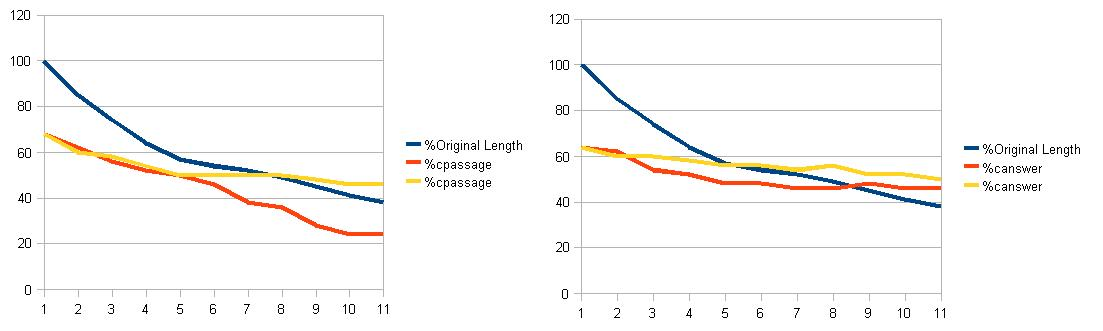
\includegraphics[scale = 0.57]{IS1008c_summaries.jpg}
%\caption{Schemas for IS1008c summaries}
%\label{schema: Results for IS1008c summaries}
%\end{figure}

\begin{table}[hb!]
 \scriptsize
\caption{Results for IB4010 summaries}
\begin{tabular}{|c|c|c|c|c|c|}
\hline
\multicolumn{ 1}{|c|}{\%Original Length \tnote{*}} & \multicolumn{ 3}{c|}{ASR Summaries} & \multicolumn{ 2}{c|}{Random Summaries} \\ \cline{ 2- 6}
\multicolumn{ 1}{|c|}{} & rank score & \%cpassage & \%canswer & \%cpassage & \%canswer \\ \hline
100 & \ensuremath{\geq0.00} & 45 & 62 & 45 & 62 \\ \hline
85 & \ensuremath{\geq0.05} & 34 & 51 & 44 & 59 \\ \hline
74 & \ensuremath{\geq0.10} & 26 & 55 & 38 & 56 \\ \hline
65 & \ensuremath{\geq0.15} & 21 & 52 & 37 & 56 \\ \hline
58 & \ensuremath{\geq0.20} & 21 & 54 & 37 & 56 \\ \hline
54 & \ensuremath{\geq0.25} & 20 & 52 & 36 & 56 \\ \hline
51 & \ensuremath{\geq0.30} & 17 & 53 & 36 & 54 \\ \hline
47 & \ensuremath{\geq0.35} & 17 & 53 & 36 & 55 \\ \hline
44 & \ensuremath{\geq0.40} & 16 & 52 & 33 & 54 \\ \hline
40 & \ensuremath{\geq0.45} & 14 & 50 & 35 & 52 \\ \hline
36 & \ensuremath{\geq0.50} & 15 & 51 & 33 & 52 \\ \hline
\end{tabular}
\begin{tablenotes}
\item[*] Original length of ASR transcript for IB4010 is 4624 words 
\end{tablenotes}
\label{tab: Results for IB4010 summaries}
\end{table}


%\begin{figure}[hb!]
%\centering
%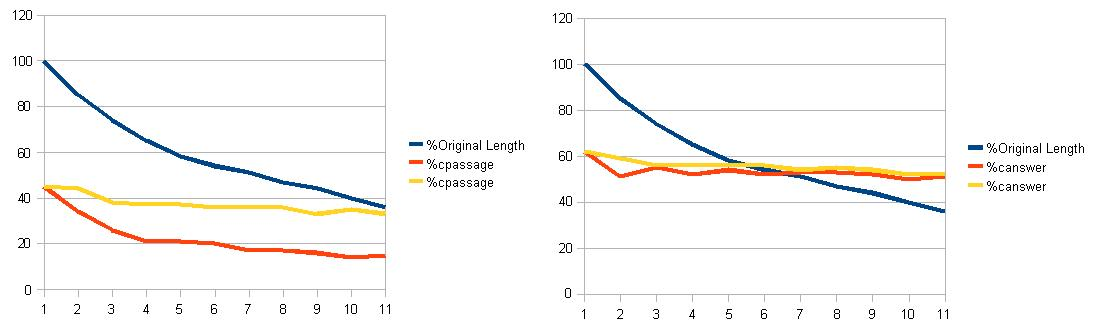
\includegraphics[scale = 0.57]{IB4010_summaries.jpg}
%\caption{Schemas for IB4010 summaries}
%\label{schema: Schemas for IB4010 summaries}
%\end{figure}


\normalsize


\section{Parameter Optimization}

The task of the parameter optimisation is to find the values for the parameters of the algorithm which are best fit for each transcript, IB4010 and IS1008c. The parameters are the search window size and search window step as a proportion of the size of the question. 

In order to do this, we used the 5-fold cross-validation method as presented in the previous chapter to build a statistic table. This table consists of columns and rows which present values of window step and values of window size correspondingly. For instance, for position (2,5), the step of search window is 2 x input question size and the size is 5 x input question size. In this table, each position (row,column) of the table presents the number of partitions as training data of the Cross-Validation method that obtain maximal scores using the value of parameters corresponding to row and column of this position. For instance, the first partition obtains maximal scores at (2,3), (2,5) and the second partition obtain maximal score at (2,4), (2,5) and the others partitions obtain maximal scores at other pairs of parameters, then value of the position (2,5) of the table is 2 corresponding to two partitions. That means when search window size is 2 and search window is 5, there are two partitions over all five partitions obtain maximal score. The maximal scores are the maximal number of true passages retrieved by the algorithm in the first phase. For this experiment, we only use the first phase Passage Retrieval because it is the most essential of the proposed algorithm.

The following tables present results obtained for IB4010 and IS1008c in detail:


 \scriptsize
\begin{center}
\begin{threeparttable}
\caption{Parameter Optimization for IB4010}
\begin{tabular}{|>{\bf}c|c|c|c|c|c|c|c|c|c|c|c|c|c|}
\hline \backslashbox{Size}{Step} & \bf{1} & \bf{2} & \bf{3} & \bf{4} & \bf{5} & \bf{6} & \bf{7} & \bf{8} & \bf{9} & \bf{10} & \bf{11} & \bf{12} & \bf{13} \\ 
\hline 1 &  &  &  &  &  &  &  &  &  &  &  &  &  \\ 
\hline 2 &  &  &  &  &  &  &  &  &  &  &  &  &  \\ 
\hline 3 &  &  &  &  &  &  &  &  &  &  &  &  &  \\ 
\hline 4 &  &  &  &  &  &  &  &  &  &  &  &  &  \\ 
\hline 5 &  &  &  &  &  &  &  &  &  &  &  &  &  \\ 
\hline 6 &  &  &  &  &  &  &  &  &  &  &  &  &  \\ 
\hline 7 &  &  &  &  &  &  &  &  &  &  &  &  &  \\ 
\hline 8 & 1 &  &  & 1 &  &  &  &  &  &  &  &  &  \\ 
\hline 9 & 4 & 3 &  &  &  &  &  &  &  &  &  &  &  \\ 
\hline 10 & 4 & 2 &	\multicolumn{1}{>{\columncolor{yellow}}c}{5}\tnote{*} &  &  &  &  &  &  &  &  &  &  \\ 
\hline 11 & 3 & 2 & 5 &  &  &  &  &  &  &  &  &  &  \\ 
\hline 12 & 1 &  &  &  &  &  &  &  &  &  &  &  &  \\ 
\hline 13 &  & 1 & 2 &  &  &  &  &  &  &  & 1 &  &  \\ 
\hline 
\end{tabular}
\begin{tablenotes}
\item[*] This position is chosen
\end{tablenotes}
\end{threeparttable}
\end{center}



\begin{center}
\begin{threeparttable}
\caption{Parameter Optimization for IS1008c}
%\begin{tabular}{|>{\bf}c|>{\sc}c|}
\begin{tabular}{|>{\bf}c|c|c|c|c|c|c|c|c|c|c|c|c|c|}
\hline \backslashbox{Size}{Step}  & \bf{1} & \bf{2} & \bf{3} & \bf{4} & \bf{5} & \bf{6} & \bf{7} & \bf{8} & \bf{9} & \bf{10} & \bf{11} & \bf{12} & \bf{13} \\ 
\hline 1 &  &  &  &  &  &  &  &  &  &  &  &  &  \\ 
\hline 2 & 1 &  &  &  &  &  &  &  &  &  &  &  &  \\ 
\hline 3 & 1 & 1 & 1 &  &  &  &  &  &  &  &  &  &  \\ 
\hline 4 & \multicolumn{1}{>{\columncolor{yellow}}c}{4}\tnote{*} & 1 & 1 & 1 &  &  &  &  &  &  &  &  &  \\ 
\hline 5 &  &  & 1 & 1 &  &  &  &  &  &  &  &  &  \\ 
\hline 6 & 2 & 2 & 3 & 1 & 2 & 1 &  &  &  &  &  &  &  \\ 
\hline 7 & 1 &  & 3 &  & 2 & 1 &  &  &  &  &  &  &  \\ 
\hline 8 &  &  &  &  &  &  &  & 2 &  &  &  &  &  \\ 
\hline 9 & 3 & 1 & 1 & 1 & 1 & 1 &  &  &  &  &  &  &  \\ 
\hline 10 & 2 &   &	1 & 1 & 1 & 1 &  &  &  & 1 &  &  &  \\ 
\hline 11 & 1 & 1 &   &  &   & 1 & 1 &  &  & 1 &  &  &  \\ 
\hline 12 & 5 & 3 & 3 &  & 2 & 4 & 3 &  &  & 1 & 1 &  &  \\ 
\hline 13 & 1 & 2 & 3 &  & 3 &   & 1 &  &  & 1 & 1 &  &  \\ 
\hline 
\end{tabular}
\begin{tablenotes}
\item[*] This position is chosen 
\end{tablenotes}
\end{threeparttable}
\end{center}

\normalsize 

According to the way of building the table above, parameters are considered good if they help as many training data as possible obtain the maximal scores. Therefore, we will choose parameters at a position whose value is the largest in the table as the relevant parameters. As seen in the table, for IB4010 there are two maximal values at (10,3) and (11,3) and for IS1008c the value of position (12,1) is the largest. These values of parameters help algorithm obtain the best scores on the training data. However, it is evident that the more the size of a search window increases, the higher the probability that a passage becomes correct. When the size of search window is equal to the size of the transcript, then it certainly contains the information of the question, so the returned "passage" (i.e. the whole meeting) always correct. In this task, we want to find parameters that help program obtain the maximal number of correct passages but the actual objective of the passage retrieval is also to decrease the search space. For this reason, we should choose the smallest size of search window that is suitable for the most partitions. That is why in the table of IS1008c, the position (4,1) is chosen. This means that the size of the search window is 4 times the question size and the step of the search window is 1 time the question size, and are thus the best fit for the BET questions and the transcript IS1008c. 
In the table of IB4010, the pair of parameters (10,3) has the best value, thus the size of search window is 10 and the step of search window is 3 and these are chosen as the best fit for the BET question and the transcript IB4010.

The chosen parameters will be used in the next section.




\section{Comparison with BET scores obtained by human subjects}

 The main goal of this comparison is to discover whether automatic machine and human subjects have the same difficulties in answering the BET questions. By analyzing the scores obtained by the system and humans, we can also identify in which case this system is useful to help humans answer the BET questions. 

The BET scores used for this comparison are results from BET for the TQB interface \cite{popescubelis2007otm} known as a Transcript-based Query and Browsing Interface. TQB is a meeting browser tool for searching and browsing multi-modal recordings of group meetings. The BET method is used to evaluate the performance of human subjects using this meeting browser over two meetings, IB4010 and IS1008c.

According to the BET method, human subjects that had not worked with TQB before were tested by answering the BET questions using TQB. They were 28 students at the University of Geneva, mainly form the School of Translation and Interpreting. Half of the subjects started with IB4010 and continued with IS1008c, and the other half did the reverse order, thus allowing for differentiated results depending on whether a meeting was seen first or second. That means when subjects worked on the first meeting, they were trained with the TQB interface, so that they answer BET questions were expected to better on the second meeting. And, indeed, the average of precision is a higher for the second meeting. In this experiment, both BET scores of the first meeting and the second meeting are used for comparison with the results obtained by the system. However, the first only 8 BET questions for each meeting are used for this comparison.  We are interested in only two pieces of information from the BET scores: average answering time and precision of each answer. 

In order to set up the configuration of the system, the parameters of search window are used from the previous section Parameter Optimisation. They are (search window size = 10 x question size, search window step = 3 x question size) for IB4010 and (search window size = 4 x question size, search window step = 1 x question size) for IS1008c.

The BET scores by human subjects and scores obtained by the system are shown in detail in two tables \ref{table: BET scores for IB4010} and \ref{table: BET scores for IS1008c}. In each table, for the scores by human subjects, \textit{Precis1} and \textit{avg time1} in seconds are average precision and average time as the first meeting, \textit{Precis2} and \textit{avg time2} are average precision and average time in seconds as the second meeting. For scores obtainned by the system, \textit{\#cpassage} and \textit{\#canswer} are the number of correct passages and the number of correct true-false answers correspondingly. However, the number of answers for each question is only one. \textit{time} in seconds is time for answering one question.




\begin{table}[htb!]
\scriptsize
\caption{Comparison with BET scores by human subjects for IB4010}
\begin{tabular}{|c|r|r|r|r|r|r|r|}
\hline
\multicolumn{ 1}{|c|}{curQuid} & \multicolumn{ 4}{c|}{Humans} & \multicolumn{ 3}{c|}{System} \\ \cline{ 2- 8}
\multicolumn{ 1}{|l|}{} & \multicolumn{1}{c|}{Precis1} & \multicolumn{1}{c|}{avg time1} & \multicolumn{1}{c|}{Precis2} & \multicolumn{1}{c|}{avg time2} & \multicolumn{1}{c|}{\#cpassage} & \multicolumn{1}{c|}{\#canswer} & \multicolumn{1}{c|}{\#time } \\ \hline
1 & 0.93 & 303.14 & 0.71 & 143 & 0 & 0 & 24 \\ \hline
2 & 0.93 & 105.36 & 1.00 & 66.14 & 1 & 1 & 22 \\ \hline
3 & 0.71 & 118.14 & 1.00 & 89.21 & 1 & 1 & 40 \\ \hline
4 & 0.86 & 207.5 & 0.86 & 206.43 & 1 & 1 & 32 \\ \hline
5 & 1.00 & 64.71 & 0.93 & 37 & 0 & 1 & 16 \\ \hline
6 & 0.93 & 57.79 & 1.00 & 53.21 & 1 & 1 & 17 \\ \hline
7 & 0.93 & 60.93 & 0.71 & 52 & 1 & 1 & 24 \\ \hline
8 & 0.71 & 129.5 & 0.79 & 85.29 & 1 & 1 & 19 \\ \hline
\multicolumn{1}{|l|}{} & \textbf{0.88} & \textbf{130.88} & \textbf{0.88} & \textbf{91.54} & \textbf{0.75} & \textbf{0.88} & \textbf{24.25} \\ \hline
\end{tabular}
\label{table: BET scores for IB4010}
\end{table}

%\begin{figure}[htb!]
%\scriptsize
%\centering
%\begin{minipage}{5cm}
%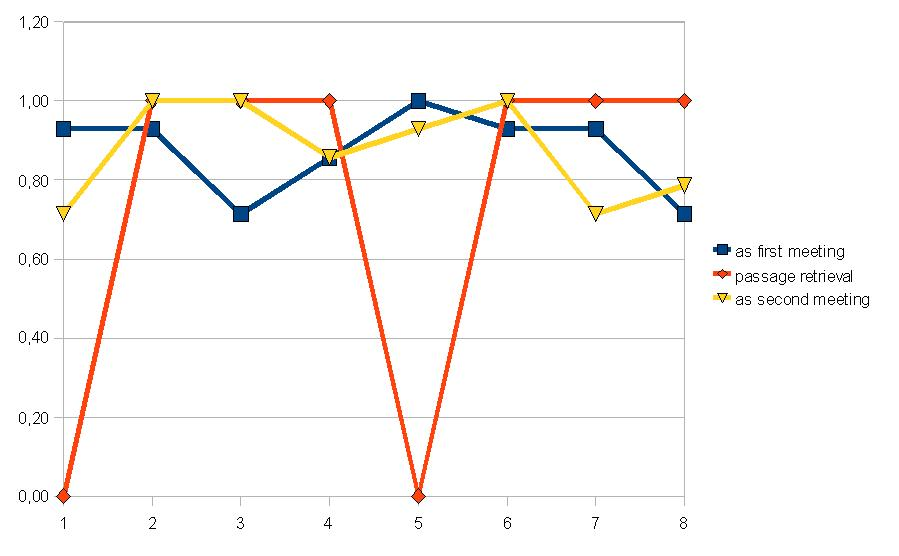
\includegraphics[width=1\textwidth]{BET_results_compararison_IB4010_passage.jpg}
%%\caption{Compararison with BET results for IS1008c (Passage retrieval)}
%\end{minipage}
%\hfill
%\begin{minipage}{5cm}
%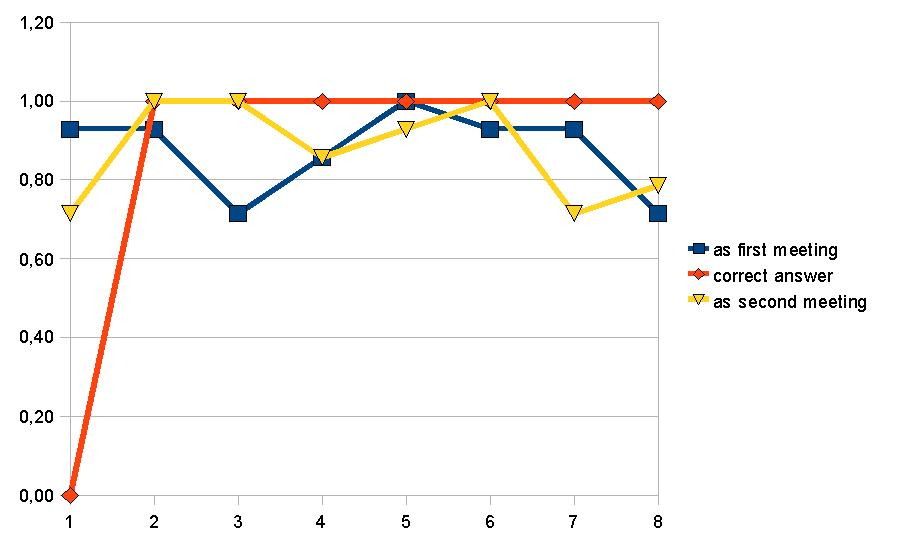
\includegraphics[width=1\textwidth]{BET_results_compararison_IB4010_truefalse.jpg}
%%\caption{Compararison with BET results for IS1008c (True-false questions answering}
%\end{minipage}
%\caption{Comparison with BET results for IB4010}
%\end{figure}
 




%Say that they come from previous study + reference

%Chu thich nguon du lieu tu BET, quota the paper on BET4TQB

According to the BET for TQB \cite{popescubelis2007otm}, average precision to answer all BET questions for IB4010 is 0.85 \ensuremath{\pm} 0.05 and 0.70 \ensuremath{\pm} 0.10 for IS1008c. For human subjects, we can divide the BET questions into two groups: "easy" and "difficult". A BET question belongs to the "easy" group  if average precision of its answers as first meeting or second meeting is more than 0.85 for IB4010 and 0.70 for IS1008c, otherwise it belongs to the "difficult" group. Meanwhile, for the system, the "easy" group includes all questions that  their number of correct passage or number of correct true-false answer is 1.
This help us have a standard to compare the BET scores by humans with scores obtainned by the system.

We first examine the results for IB4010. According to the convention above, for human subjects there is only one "difficult" question (question number 8), while there are two "difficult" questions for the system (questions number 1 and 5). In fact, all of these questions are \textit{deductive questions} that require deep comprehension rather than a search of lexical similarities. For the question number 1, the true and the false statement in this pair are "The group decided to show The Big Lebowski" and "The group decided to show Saving Private Ryan" respectively. This question requires to read all of the transcript before answering the question. That is why the system could not identify the correct passage using a small search window that does not cover all the information of the transcript as it requires for this type of question. Consequently, the true-false answer is determined by chance (false in this case). The question number 5 also requires a deduction to distinguish the true statement "No one had seen Goodfellas" from the false statement "Everyone  had seen Goodfellas". In the meeting, when all meeting participants said "No" for the question "Have you seen Goodfellas?", it is easy for human subjects to understand the answer of the participants. However, this is really a difficult task for an automatic system.  The system identified the incorrect passage. Consequently, its true-false answer is determined by chance, that is true in this case. Question number 8, whose the true and the false statement are "Agnes eliminates Pulp Fiction as she dislikes Quentin Tarantino" and "Agnes eliminates Pulp Fiction as it is too violent" is also a deductive question because it is not easy to match the question "I dislike Quentin" with the text "I am not a huge fan of Quentin Tarantino". However, the system gave the true answer for this question while it was difficult for human subjects. That is because the keyword Quentin appears only one time in the transcript and the system was based on this word, but not based on the meaning of the essential phrase to identify the correct passage.

\begin{table}[ht!]
\scriptsize
\caption{Comparison with BET scores by human subjects for IS1008c}
\begin{tabular}{|c|r|r|r|r|r|r|r|}
\hline
\multicolumn{ 1}{|c|}{curQuid} & \multicolumn{ 4}{c|}{Humans} & \multicolumn{ 3}{c|}{System} \\ \cline{ 2- 8}
\multicolumn{ 1}{|l|}{} & \multicolumn{1}{c|}{Precis1} & \multicolumn{1}{c|}{avg time1} & \multicolumn{1}{c|}{Precis2} & \multicolumn{1}{c|}{avg time2} & \multicolumn{1}{c|}{\#cpassage} & \multicolumn{1}{c|}{\#canswer} & \multicolumn{1}{c|}{\#time} \\ \hline
1 & 0.86 & 410 & 0.93 & 127.36 & 1 & 1 & 13 \\ \hline
2 & 0.67 & 298.58 & 0.86 & 129.5 & 1 & 1 & 45 \\ \hline
3 & 0.82 & 78.09 & 0.93 & 67.5 & 1 & 1 & 15 \\ \hline
4 & 0.89 & 80.22 & 0.93 & 103.93 & 1 & 1 & 16 \\ \hline
5 & 0.63 & 66.38 & 0.69 & 63.92 & 1 & 0 & 20 \\ \hline
6 & 0.67 & 44 & 0.73 & 62.18 & 0 & 0 & 10 \\ \hline
7 & 1.00 & 24 & 0.82 & 48 & 1 & 0 & 11 \\ \hline
8 & 0.67 & 66 & 0.64 & 93.55 & 0 & 1 & 11 \\ \hline
\multicolumn{1}{|l|}{} & \textbf{0.77} & \textbf{133.41} & \textbf{0.81} & \textbf{86.99} & \textbf{0.75} & \textbf{0.63} & \textbf{17.63} \\ \hline
\end{tabular}
\label{table: BET scores for IS1008c}
\end{table}

For IS1008c, as defined above, for "easy" and "difficult" questions there are two "difficult" questions for human subjects. They are questions numbered 5 and 8. For the system, it incorrectly answered three questions that are questions numbered 5, 6,7 and 8, in which the questions numbered 5, 6 and 8 are deductive questions. For question numbered 5, whose the true statement is \textit{Agnes express her opinion that ...}, the correct passage should be \textit{Agnes: I think ... }. Two different expressions make it difficult to understand for both human subjects and the automatic system. With regard to question number 6, whose the true statement is "Agnes notes some reasons to not have a display" and the false statement is "Agnes tries to persuade the group they should have a display", Agnes showed a list of reasons in the transcript but there is few matched words between question string and answer string. This is similar with question number 8, which has the true statement and the false statement are "Market research suggests the remote has to be new and different." and "Market research suggests the remote has to be comfortable and familiar." respectively. However, the true-false answer for question numbered 8 is correct by chance. Question number 7 is not difficult. It has the true statement and the false statement are "Ed commented that they had a product but that cost was going to be a potential problem" and "Ed commented that they had a product and that cost was not going to be a problem" respectively. For this question the system gave correct passage but incorrect true-false answer. That means true-false answers by the system are not as stable as correct passage answering.

In conclusion, although both human subjects and the system encounter difficulties to answer deductive questions, these are more difficult for the automatic system. For IB4010, there are 3 deductive questions and the automatic system incorrectly answered 2 out of 3 questions, while at the same time, the human subjects have difficulty only answering 1 of the 3 questions. For IS1008c, there are also 3 deductive questions. The system gave the wrong answers for all three questions, meanwhile the human subjects had difficulty answering two questions. In fact, deductive questions are equivalent to How and Why questions that are difficult for all question answering systems \cite{prager2000qap, brill2002diq}.

According to the experimental results, the results for the passage retrieval are more logical than the results for true-false answers. That means the system should be developed to help humans answer BET-typed questions by identifying relevant passage instead of giving the final answers. In other words, it is a useful tool for locating the answer, but not necessarily for answering questions directly \cite{lequocanh1}.
 

\newpage










\chapter{Conclusion and future works}

The performance of the automatic true-false question answering system is quite below that of humans using existing browsers. However, the scores of passage retrieval stage are a lot better  than random scores, are obtained in a very short time (less than 1s per question).

The human subjects answer questions that require a deduction or a reflexion better than the system does, but the system gives the answers much more quickly. Thus, the automatic system should give consultative information for a question given by users rather than return the answer in a fully autonomous way.

In conclusion, this project opens a new starting point to develop a fully-automatic question-answering system for meeting browsers. The lexical similary methodology may not be able to solve completely this problem. Nevetheless, it is an open problem and need further researches. 
%Within 6 months of doing this project, I do not have ambition to study
%and find out a perfect solution but try to experience with simple and basic one.

%%%%%%%%%%%
\section*{Future works}
The results of the passage retrieval propose a promising assistant tool for meeting browsers. This automatic tool integrated into a meeting browser could help users locate relevant information in a short amount of time so that they can save time to reason out the answer to a question.

This is the first attempt for building an automatic meeting browser following to question answering approach. Thus, this system can be developed by adding a \textit{answer extraction} stage after the passage retrieval stage in order to extract a short phrase that expresses the answer instead of giving an answer \textit{true} or \textit{false}. However, this requires more significant research on semantic analysis of texts and dialogues.

\chapter*{Appendix}
\addcontentsline{toc}{chapter}{Appendix}

\section{Results for Cross-Validation}


\begin{figure}[hb!]
\centering
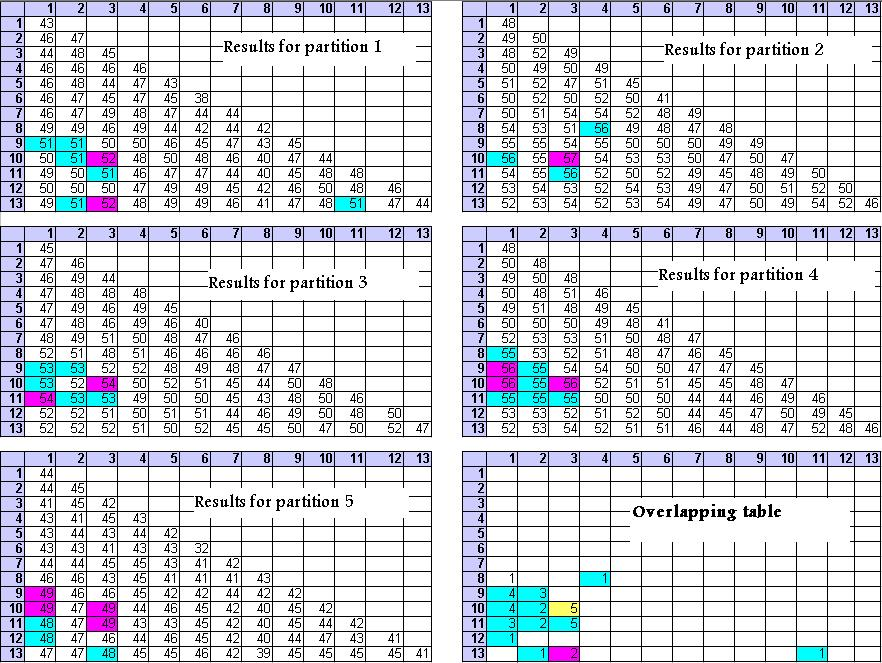
\includegraphics[scale = 0.85]{IB4010_optimisation.jpg}
\caption{Using 5-fold Cross-Validation for parameter optimisation for IB4010}
\label{Using 5-fold Cross-Validation for parameter optimisation for IB4010}
\end{figure}

\pagebreak


\begin{figure}[hb!]
\centering
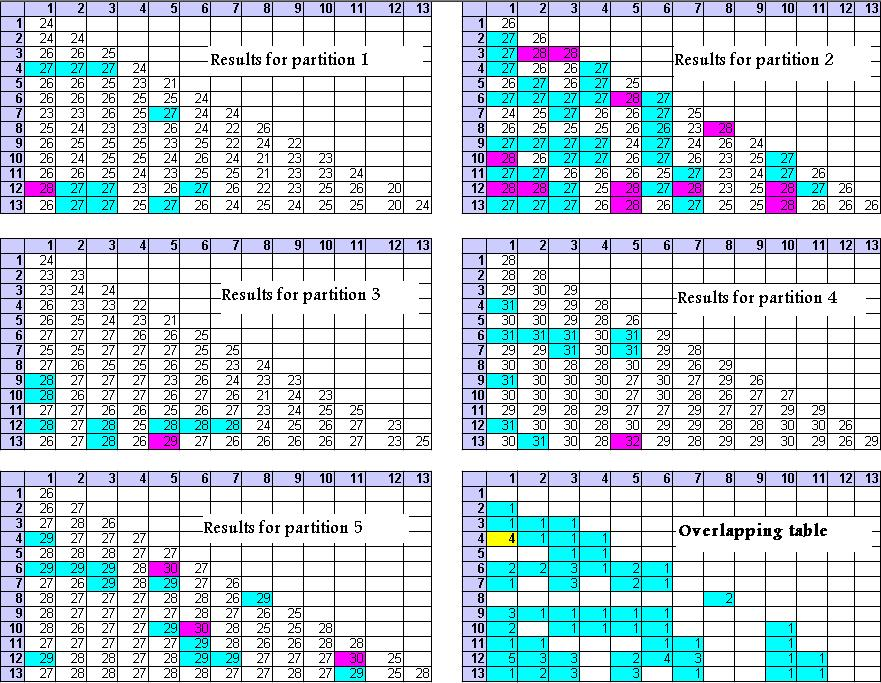
\includegraphics[scale = 0.85]{IS1008c_optimisation.jpg}
\caption{Using 5-fold Cross-Validation for parameter optimisation for IS1008c}
\label{Using 5-fold Cross-Validation for parameter optimisation for IS1008c}
\end{figure}

The two figures above show the results in detail for the section Parameter Optimization over the meetings, IB4010 and IS1008c. Following the Cross-Validation method, the set of questions is divided into 5 partitions and the results for each partition are described in the figures. There are 6 tables for each meeting in which 5 tables contain the results for 5 partitions correspondingly and the last table contains the collected results from 5 partitions. The row and the column of each table are the step and the size of search window. In the 5 tables for the results of partitions, the value of each cell is the average number of correct passages for the subset of questions with the parameters corresponding to the row and the column. Meanwhile, in the last table, the value of each cell is the number of the highest values from 5 partitions overlapped for the same parameters.

%What goes in the appendices? Any material which impedes the smooth development of your
%presentation, but which is important to justify the results of a thesis. Generally it is material
%that is of too nitty-gritty a level of detail for inclusion in the main body of the thesis, but which
%should be available for perusal by the examiners to convince them sufficiently. Examples include
%program listings, immense tables of data, lengthy mathematical proofs or derivations, etc.

%\section{Source code in Java}
%\subsection{Calculating passage score}
%
%\lstset{numbers=left, stepnumber=1,breaklines=true}%,basicstyle=\footnotesize ,numberstyle=\footnotesize , showspaces=false, showstringspaces=false, showtabs=false, breakatwhitespace=true }
%
%\lstset{language=Java, caption=Calculating Passage Score, label=DescriptiveLabel}
%\lstset{frame=shadowbox, rulesepcolor=\color{blue}}
%%\begin{frame}
%\lstinputlisting{code.java}
%%\end{frame}
%
%
%\section{Source code of the procedure Determining True Statement}
%%\begin{framed}
%%\begin{lstlisting}…\end{lstlisting}
%%or \lstinputlisting{…}
%%\end{framed}


\section{List of stopwords}
The stopwords that were removed from the transcripts and the questions are listed below. 

\small 
\textit{i, a, about, above, an, are, as, at, am, and, be, been, being, but, by, do, does, done, did, for, he, her, hers, herself, his, him, himself, how, in, is, it, its, itself, me, my, mine, myself, nor, of, on, or, our, ours, ourself, ourselves, so, she, that, the, they, them, their, theirs, these, themself, themselves, this, those, to, uh, um, up, us, really, very, was, were, we, well, will, with, what, when, where, which, who, whom, whose, why, yet, you, your, yours, yourself, yourselves.
}
\normalsize

\pagebreak

\section{Part-of-speech tags}

\begin{table}[htbp]
\scriptsize
\caption{POS tags used by the QTAG tagger}
\begin{tabular} {|lp{4cm}|lp{4cm}|lp{8cm}|lp{0cm}|} %{|l|l|l|l|}
\hline
\textbf{POS } & \textbf{description } & \textbf{POS } & \textbf{description } \\ \hline
BE & be & PN & pronoun, indefinite \\ \hline
BEDR & were & POS  & possessive particle \\ \hline
BEDZ & was & PP & pronoun, personal \\ \hline
BEG & being & PP\$ & pronoun, possessive \\ \hline
BEM & am & PPX & pronoun, reflexive \\ \hline
BEN & been & RB & adverb, general \\ \hline
BER & are & RBR & adverb, comparative \\ \hline
BEZ & is & RBS & adverb, superlative \\ \hline
CC & conjunction, coordinating & PP & adverbial particle \\ \hline
CD & number, cardinal & SYM & symbol or formula \\ \hline
CS & conjunction, subordinating & TO & infinitive marker \\ \hline
DO & do & UH & interjection \\ \hline
DOD & did & VB & verb, base \\ \hline
DOG & doing & VBD & verb, past tense \\ \hline
DON & done & VBG & verb, -ing \\ \hline
DOZ & does & VBN & verb, past participle \\ \hline
DT & determiner, general & WBZ & verb, -s \\ \hline
EX & existential there & WDT & det, wh- \\ \hline
FW & foreign word & WP & pronoun, \\ \hline
HV & have & WP\$ & pronoun, possessive \\ \hline
HVD & had & WRB & adv, wh- \\ \hline
HVG & having & XNOT & negative marker \\ \hline
HVN & had & ! & exclamation mark \\ \hline
HVZ & has & ' & quotation mark \\ \hline
IN & preposition & ' & apostrophe \\ \hline
JJ & adjective, general & ( & parenthesis begin \\ \hline
JJR & adjective, comparative & ) & parenthesis end \\ \hline
JJS & adjective, superlative & , & comma \\ \hline
MD & modal auxiliary & - & dash \\ \hline
NN & noun, common singular & . & point \\ \hline
NNS & noun, common plural & ... & ... \\ \hline
NP & noun, proper singular & : & colon \\ \hline
NPS & noun, proper plural & ; & semi-colon \\ \hline
OD & number, ordinal & ? & question mark \\ \hline
PDT & determiner, pre- & ??? & undefined \\ \hline
\end{tabular}
\label{PoS}
\end{table}


%\newpage




\chapter*{Glossary}   
\addcontentsline{toc}{chapter}{Glossary}

\small

\begin{itemize}
\item {Stem: A stem or word stem is a root or roots of a word that is common to all its inflected variants \cite{Stem}. }

\item {Lemma: A lemma in morphology is defined as a canonical form of a set of words that have the same original meaning \cite{clement2004mba}. A lemma is different from a stem in which a lemma of the verb may change when morphologically inflected, however a stem that never changes by doing a morphology. For example, for the word "modified", its lemma is "modify" while the stem is "modifi" because we have words such as \textbf{modifi}cation (verified by WordNet\cite{miller1995wld})}

\item {Morphology: The morphology of the language is defined in terms of a set M of relations between word forms \cite{miller1995wld}}

\item {Keyword: In our system, a keyword is defined as any important word that will help an automatic machine answer a question \cite{buscaldi2007ngv}}

\item {Part-of-speech tagger: A programme determines the identification of a word as a noun, a verb, an adjective,... based on definition of the word and the sentence that the word belongs to. \cite{manson1997qpp}}

\item {Stopword: It is a word such as "the", "to" or "for" which generally add little or no information regarding the subject matter of a document \cite{mckechnie2001cap}}

\item {Punctuation marks: According to Todd, Loreto (2000),  punctuation marks are everything in a text other than the letters or numbers.}

\item {Synonym: A synonym of a word is another word that they share at least one sense in common \cite{miller1995wld}. }

\item {Dynamic Search Window: That is a window used for block-matching algorithm in information retrieval by moving this window to all data blocks as possible. A dynamic search window has dynamic parameters (size and step) that depend on input data. \cite{goharian2008dsp}. In our case, a window moves to all passages as possible in the transcript to retrieve a relevant passage.}

\item {Passage: A passage can simply be defined as a sequence of words regardless of sentences or paragraphs. Some text-based information retrieval systems define a passage as a fixed-length block of words \cite{goharian2008dsp}.}

\item {Passage Score: In text-based question answering system, the score of a passage is based on the score of its words with respect to question words. The score of a question word found in a passage is computed based on definition of this word and/or relations of this word with other words in the text \cite{tellex2003qep}.}

\item {Passage Retrieval Algorithm: Its objective is to determine a passage that is the most likely to contain information that helps for answering a question \cite{tellex2003qep}.}

\item {Meeting Browser:  A tool that help humans find relevant information from past meetings in multimedia archives of meeting recordings \cite{popescubelis:tbe}.}

\item {BET: Browser Evaluation Test. This is a method for assessing the performance of a meeting browser on meeting recordings \cite{BET}.}

\item {Observation of interest: They are statements about a fact related to a meeting collected by independent observers in order to perform an evaluation for meeting browsers according to the Browser Evaluation Test (BET) method \cite{BET}.}

\item {Observers: They watch selected meetings from corpus, to produce a set of \textit{observations of interest}}.

\item {BET Questions: They are questions used in  the BET method \cite{popescubelis:tbe}.}

\item {Human Subjects: They are persons who answer BET questions using a meeting browser \cite{BET} and their answers are used to evaluate the performance of this browser.}

\item {Corpus: A set of meeting recordings }

\item {Question-Answering System: A text-based system that allows users to  ask a question in natural language and receive an exact and succinct answer in place of a list of documents that may contain the answer \cite{hirschman2002nlq, kato2004hia}.}

\item {Deductive Question: Firstly, it comes from the difference expression between strings from question and strings from answer. This is the biggest challenges for question answering \cite{brill2002diq}. Secondly, this question type demands to seek a fact rather a clear explanation in the text, for example for "How" and "Why" questions. They are difficult for all question answering systems \cite{prager2000qap}.}

 
\item {ASR meeting transcript: Meeting transcripts are generated by Automatic Speech Recognition \cite{BET}.}

\item {ASR summaries: They are generated by an automated summarizer based on ASR meeting transcripts \cite{ASR_summaries}.}

\item {Cross-Validation method: This method is used to test a configuration of a system for an accuracy estimation in the case that the system does not have enough data to test \cite{kohavi1995scv}.}

\item {N-gram matching: In textual information retrieval, this method is used to estimate similarity between two string by examining all n-grams matchings, where an n-gram is a substring of n words \cite{robertson1998ang}.}

\item {TREC: The Text Retrieval Conferences \url{http://trec.nist.gov/}. This is an series of workshops for a list of different information retrieval research which question answering belongs to.}

\end{itemize}

\normalsize






\label{Bibliography}

%\lhead{\emph{Bibliography}}  % Change the left side page header to "Bibliography"
\bibliographystyle{unsrtnat}  % Use the "unsrtnat" BibTeX style for formatting the Bibliography
%\clearpage

\bibliography{biblio}  % The references (bibliography) information are stored in the file named "biblio.bib"
\addcontentsline{toc}{chapter}{Bibliography}



%\bibliographystyle{plain}	% (uses file "plain.bst")
%\bibliography{biblio}		% expects file "myrefs.bib"


\end{document}